\documentclass[twoside,11pt]{article}
\usepackage{jair, theapa, rawfonts}

\jairheading{x}{20xx}{xx}{xx}{xx}
\ShortHeadings{Participatory Budgeting  Designs for the Real World}
{Fairstein, Benad\`{e}, Gal}
\firstpageno{1}
 
\usepackage[hyphens]{url}  % DO NOT CHANGE THIS
\usepackage{graphicx} % DO NOT CHANGE THIS
\urlstyle{rm} % DO NOT CHANGE THIS
\def\UrlFont{\rm}  % DO NOT CHANGE THIS
%\usepackage{natbib}  % DO NOT CHANGE THIS AND DO NOT ADD ANY OPTIONS TO IT
\usepackage{caption} % DO NOT CHANGE THIS AND DO NOT ADD ANY OPTIONS TO IT
\frenchspacing  % DO NOT CHANGE THIS
\setlength{\pdfpagewidth}{8.5in} % DO NOT CHANGE THIS
\setlength{\pdfpageheight}{11in} % DO NOT CHANGE THIS

\usepackage{xcolor}
\usepackage{color,soul}
\usepackage{amsmath}
\usepackage{amssymb}
\usepackage{mathtools}
\usepackage{cleveref}
\usepackage{longtable}
\usepackage{makecell}
\usepackage{subcaption}

\newcount\Comments  % 0 suppresses notes to selves in text
\Comments=1
\newcommand{\kibitz}[2]{\ifnum\Comments=1{\color{#1}{#2}}\fi}
\newcommand{\rf}[1]{\kibitz{blue}{[Roy says:#1]}}
\newcommand{\kg}[1]{\kibitz{brown}{[Kobi says:#1]}}
\newcommand{\gb}[1]{\kibitz{red}{[GB:#1]}}
\newcommand{\ns}[1]{\kibitz{purple}{[Nisarg:#1]}}

\newcommand{\points}{\textsc{Points}}
\newcommand{\rank}{\textsc{Rank}}
\newcommand{\vfm}{\textsc{Vfm}}
\newcommand{\knap}{\textsc{Knap}}
\newcommand{\kapp}{\textsc{Kapp}}
\newcommand{\tapp}{\textsc{Tapp}}
\newcommand{\sw}{\textsc{sw}}
\newcommand{\voters}{{N}}
\newcommand{\mes}{ES}
\newcommand{\pabu}{PaBuLib}



\begin{document}

\title{Participatory Budgeting  Designs for the Real World}

\author{\name Roy Fairstein \email royfa@post.bgu.ac.il \\
       \addr  Ben-Gurion University of the Negev, Israel
       \AND
       \name Gerdus Benad\`{e} \email benade@bu.edu \\
       \addr Boston University, MA, USA
       \AND
       \name Kobi Gal \email kobig@bgu.ac.il \\
       \addr Ben-Gurion University of the Negev, Israel \\
       University of Edinburgh, UK }

% For research notes, remove the comment character in the line below.
% \researchnote

\maketitle


\begin{abstract}
  Participatory budgeting (PB) is a type of crowdfunding which engages the inhabitants of a city  in the process of allocating  public money to different types of projects. 
  PB processes  differ in how voters are asked to express their preferences over candidate projects and how these preferences are aggregated to determine which projects to fund. 
  This paper studies  two fundamental questions in PB design: which voting format and aggregation method to use?
  We conduct an extensive experiment in which $1\,800$ participants vote in four participatory budgeting elections in a controlled setting to evaluate the practical effects of the choice of voting format and aggregation rule. 
    We find  that $k$-approval leads to the best user experience. 
    With respect to the aggregation rule, we focus on stability, or the robustness of the rule to the choice of input format and partial participation. Greedy aggregation leads to outcomes that are  highly sensitive to   the input format used and the fraction of the population that participates. The method of equal shares, in contrast, leads to outcomes that are not sensitive to the type of voting format used, and these outcomes are remarkably stable even when the majority of the population does not participate in the election.  This finding is  replicated on data from a repository of nearly 500 real participatory budgeting elections. 
\end{abstract}


%\cite\shortcite

\section{Introduction}\label{sec:intro}
%alternative
% PB process + spreading, cool and exciting
% but it faces some challenges - low participation
% in light of this, design is important, balance many factors. Elicitation + aggregation
% Elicitation + discussion
% aggregation + discussion


Participatory budgeting (PB) is an exciting form of direct democracy that allows a community to take part in deciding how to allocate a budget among different projects. 
%It is growing in popularity and has been used around the world including in major cities like Madrid, Rome, Paris~\cite{sintomer2008participatory} and New York~\cite{su2017porto}.  One benefit of participatory budgeting is that it can increase community satisfaction by allowing voters to affect local decisions that matter to them. 
%allows voters to affect local policies that matter to them, and  can increase community satisfaction when  better sets of projects are funded. 
%
A participatory budgeting election  consist of several phases. First, organizers elicit proposals for  projects. These proposals are developed further (expanded, merged, costed, etc.) and finally filtered to a set of candidate projects.  Citizens are then asked to cast a vote which expresses a preference over the candidate projects, and the votes are aggregated to determine which projects are funded.
%
Participatory budgeting is growing in popularity around the world, in part because it empowers communities to have a direct say on local policies that affect them,  and it has been used  in major cities like Madrid, Rome, Paris and New York~\cite{sintomer2008participatory,su2017porto}.  %One benefit of participatory budgeting is that it can increase community satisfaction by allowing voters to affect local decisions that matter to them. 

%Like most democratic innovations, participatory budgeting also faces very real challenges. 
Despite the early success of participatory budgeting and its increasing adoption over the last two decades, it also faces very real challenges. 
For example, participation rates in PB elections are often low, in  extreme cases as low as 0.1\% in Germany~\cite{zepic2017participatory} and 1-3\%   in Chicago in 2012 and 2014~\cite{stewart2014participatory,carroll2016democratizing}. 

We study the complex task of  designing  participatory budgeting elections that are inclusive, easy to participate in, and produce high quality outcomes.   In particular, we assume that a shortlist of candidate projects have been fixed through some process and focus on the latter two components of the election: \emph{preference elicitation}, or how voters are asked to express their preferences, and \emph{aggregation} --- how votes are aggregated to determine which projects to fund. 


In terms of preference elicitation,   voters should be able to express complex preferences over projects, for example, a voter may   prefer exactly one library being built rather than zero or two libraries, while being indifferent between the two proposed locations. At the same time, voting should be accessible to everyone  no matter their educational or socio-economic background, and there is a real risk that requiring too much information from voters can deter   participation. 
Very simple voting formats, on the other hand,   come with their own problems and can lead to frustration and disillusionment. 
Organising bodies  may also have secondary objectives, for example, designing an input format which exposes voters to   budgetary constraints similar to what the city council faces.  
%
The vast majority of real-world PB elections use $k$-approval voting \cite{aziz2021participatory}, in which a voter approves their most preferred $k$ projects, though we are we aware of little formal justification for this choice.  Other formats that have been proposed in the literature or used in practice include knapsack voting (voters approve their most preferred budget-feasible set)  \cite{goel2019knapsack}, ranking projects by value or value-for-money  \cite{aziz2020expanding,benade2021preference} and reporting (typically additive)  utilities \cite{peters2021proportional}. 

When it comes to aggregation,  the funded projects should   reflect the preferences of  as large a part of the population as possible. Outcomes are commonly evaluated in terms of \emph{social welfare}, using some proxy for voter utility functions derived from their votes, and \emph{representation}, which tries to capture whether the preferences of every subgroup in the population (for example, each neighbourhood) contributed to the outcome in proportion  to the subgroup's size.
In light of low real-world turnout at participatory budgeting elections, we posit that another desirably property of an aggregation rule is a form of \emph{stability}, or robustness. 
We distinguish between two forms of stability. In the first, the outcome of the election is robust to the choice of input format --- this allows the organizers to freely select an input format without fear of affecting the outcome of the election. In the second, the outcome of the election is robust to partial participation --- voter turnout may be low in real PB elections, ideally the outcome of the election is not drastically affected by the {(non-)participation} of a potentially sizable random   group of   voters. 
%
Real-world elections almost exclusively use some form of greedy aggregation in which projects are selected in decreasing order of the number of approvals   received. The Method of Equal Shares (\mes{})~\cite{peters2021proportional}, which was used in elections in Switzerland and Poland in 2023,  is perhaps the only real challenger to greedy aggregation.
Alternatives like Cumulative Single Transferable Vote~\cite{skowron2020participatory} and variations on the greedy approach~\cite{talmon2019framework}   are yet to be of practical significance.



We perform   a comprehensive  study of the effect of voting format and aggregation rule on  both the voter experience and the quality of the resulting outcomes    towards answering the fundamental design question of
\emph{what input format and aggregation method should be used  in participatory budgeting elections?
}

\subsection{Our Contributions}

%corporate fundraising  - GOrd

Our study consists of two parts: a user experiment    with more than $1\,800$ participants, and a computational study using publicly available data from nearly 500 real participatory budgeting elections. 

We recruit more than $1\,800$ participants on Amazon Mechanical Turk (MTurk),  present each with one of four different PB elections  and ask them to vote in one of six   input formats. 
We track several aspects of the voter experience, including the time it takes to learn and use each format and voters' self-reported belief that an input format accurately captures their preferences.  
%
We find that $k$-approval voting leads to the best voter experience. Voters using $k$-approval spent the least time  learning the format and casting their votes and found the format easiest to use. Somewhat surprisingly, voters also felt that  it was the format that allowed them to express their preferences best, despite the fact that $k$-approval captures strictly less information about voter preferences than, for example,  a ranking of the projects. 


We compare the outcomes from using greedy aggregation and \mes{} on the votes cast during the MTurk experiment. Throughout our evaluation we use the most common ways of associating votes with utilities from the literature: for   ranking-based input formats we use Borda scores, and for the approval based formats we use both binary (\{0,1\}) and cost (\{0, cost\}) utilities.
We find no significant difference in   social welfare and representation of these rules.  
We define a new notion of entropy to measure stability and    %\footnote{We also attempt to compare the social welfare of the outcomes from different aggregation methods and don't find significant differences. Refer to the appendix for further details. }  %Although the two methods lead to comparable social welfare, we identify two  advantages of \mes{} over greedy aggregation.
 find that \mes{} has two advantages over greedy aggregation on this axis. 
First, it is much less sensitive to the input format used --- no matter the input format used, the set of projects that are funded remains almost identical. This makes \mes{} very versatile: as long as \mes{} is used for aggregation, the designer can choose almost any reasonable input format to satisfy whatever secondary objectives are present without fear that this will distort the outcome of the election. Second, we find that \mes{} is remarkably stable as participation decreases. In fact, sampling as few as 25-50\% of the voters and aggregating only the sampled votes rarely leads to a change in the set of projects being funded. In light of low levels of real-world participation, we believe this is a particularly attractive property (and one  not shared by greedy aggregation).

Next, we investigate whether our finding that \mes{} is more stable than greedy aggregation can be replicated outside the confines of our user experiment. We use publicly available data from \pabu{} from 4xx real-world participatory elections. These elections have up to XXXX voters and YYYY projects, and voters cast approval votes. 
We mimic partial participation by repeatedly sampling a small fraction of the  votes cast in each election, aggregating the sample and tracking the outcome. 
On small instances with less than 10 projects and those that are tightly constrained, in the sense that at most two randomly selected projects can be funded, there is little difference in stability between \mes{} and greedy aggregation. However, on larger instances where there is more flexibility and a greater number of feasible outcomes, \mes{} is consistently and significantly more stable than greedy aggregation. This finding does not depend on the choice of utility model. %holds  on both the most common ways of associating approval votes with utilities.  whether you convert approval votes to binary (\{0,1\}) or cost (\{0, cost\}) utilities, the two most commonly assumed. 

Our study provides a structured comparison of participatory budgeting design choices with valuable insights for   practitioners. 
The data set collected during the user experiment is publicly available; we  hope that it will benefit future research.  % Our dataset and code will be made publicly available. 
 
 
\section{Related Work }\label{sec:related}
%ibm stuff, homebias in crowd funding

We briefly remark on the most closely related work; for a thorough review of the participatory budgeting literature see \shortcite{aziz2021participatory}.

Our work is closest to  \shortcite{benade2018efficiency}, who study the role of input formats in lab controlled PB settings. They asked participants  to vote over items that may aid their survival in a desert island. Each item has an associated weight and participants are informed that they are only able to carry items up to a specified weight limit. 
\shortcite{benade2018efficiency} report on the time it takes to vote, the consistency of preferences across format, and the distortion and welfare of different aggregation methods (under the assumption that the utility of an alternative is equal to the points assigned to it).
In their work voters face only a single set of alternatives, and the desert island framing is far removed from PB as practiced in cities.  It is  hard  to argue that their findings are general  (for example, there may just be an obvious budget-feasible set of projects that best aids survival).   Our experiment much more closely mimics real-world participatory budgeting elections by using projects from real elections and  locating projects on a city map. We   attempt to check the robustness of our findings by repeating the experiment across four elections with different sizes and projects. 
\shortcite{goel2019knapsack} propose knapsack votes and empirically compare       value-for-money comparisons, knapsack and $k$-approval votes in several ways, including through a user survey. It is found that knapsack and $k$-approval votes take a similar amount of time, while value-for-money comparisons induce less cognitive load.  We find the opposite: voters consistently take significantly longer to  form value-for-money rankings. One possible explanation is that \shortcite{goel2019knapsack} performed a pair-wise comparison between projects, while we ask the voters for a full ranking over all projects. \shortcite{goel2019knapsack}   show some theoretical properties of knapsack under overlap utilities. 

\shortcite{benade2021preference}  study the theoretical information content of different input formats in a worst-case model.
They also conduct simulations, using votes from real PB elections,  to evaluate the social welfare that result from different input formats under a particular aggregation rule. They found that ``threshold approval" had both the strongest theoretical guarantees and highest welfare in simulations. 
Threshold approval does not stand out in our results.

A large literature studies the axiomatic properties of aggregation rules. Analysis most often focuses on maximizing the social welfare of the outcome \cite{benade2021preference,goel2019knapsack,jain2020participatory,hershkowitz2021district,talmon2019framework} %\gb{other papers that maximize welfare?} 
or satisfying some version of proportionality, which (roughly) requires that a group of voters  with similar opinions should have impact on the outcome proportional to the size of the group \cite{fain2016core,aziz2017justified,sanchez2017proportional,fain2018fair,aziz2018proportionally,skowron2020participatory,peters2021proportional} or both \cite{fairstein2022welfare,michorzewski2020price}.  Notably, \mes{} satisfies a proportionality condition called extended justified representation that guarantees a degree of representation to minority groups with common interests \cite{PS20}. 

We briefly look at welfare and representation but focus on evaluating  the stability of greedy aggregation and \mes{}, which  concerns the degree to which the outcome changes as one varies either the input format used in the election, or the degree of participation.  To the best of our knowledge this has not been studied before. 

\gb{todo stability link to  manipulatbility}\rf{I assume you mean link between responsiveness and manipulability}




\section{Preliminaries}\label{sec:prem}

For   $k\in \mathbb{N}$,  let $[k] := \{1,\ldots,k\}$. A PB instance is defined by a set of $n$ voters $N=[n]$ that express their preferences over a set of $m$  projects $P=[m]$ and a budget $B$. 
Each project  $p\in P$ has cost   $c(p)$. 
The purpose  of  a participatory budgeting process  is to select  a subset of projects $S\subseteq P$  to fund which satisfies the budget constraint, so $c(S) =  \sum_{p\in S} c(p) \leq B$. 


We assume that voter $i$ gains utility $v_i(p)$ from project $p$ being funded. The value that  voter $i$ has for a set of projects $S\subseteq P$ is $v_i(S) = \sum_{p\in S} v_i(p)$, i.e. we assume additive utilities. 
The social welfare of project $p$ is $ v(p) = \sum_{i \in \voters} v_i(p)$ and the social welfare of outcome $S$ is $\sw(S) = \sum_{i\in \voters} v_i(S) = \sum_{p \in S} v(p).$ 

In reality, we do not have access to voters' true utilities. Instead, we receive a vote cast in some input format as proxy for these utilities. We study the following input formats.
% %We assume voters have normalized, additive utility functions and 
% The PB literature has   suggested different input formats that voters can use to 
% express their preferences over projects. We list the most common input formats below.
% %that they are able to express their preferences in one of six ways: 
\begin{enumerate}
    \item A \textit{utilities}  vote  (referred to as \points) asks a voter to divide 100 points between projects. Voter $i$ assigns $u_i(p) \in \mathbb{N}_0$ to each project $p\in P$ so that $\sum_{p\in P} u_i(p) =100. $ 
    %This is the most straightforward way to express preferences, but prior research has shown that people do not excel at assigning the correct utilities to choices.\kg{citation}
       
     \item  A \textit{$k$-approval}   vote (\kapp) asks a voter to approve (up to) their  $k$ most preferred projects. The $k$-approval vote of voter $i$ is represented as a binary vector $\alpha_i\in\{0,1\}^m$ with $\sum_{p\in P}\alpha_i(p)\leq k$.
      
    
    \item A \textit{threshold approval} vote  (\tapp) with threshold $t$ asks a voter to approve projects for which they have utility  at least $t$.  Voter $i$'s preferences are represented by a  binary vector $\alpha_i\in\{0,1\}^m$. 
    
    \item A \textit{knapsack} vote  (\knap)   asks each voter to select a subset of projects to maximize their utility subject to the budget. Voter $i$'s vote is a binary vector $\alpha_i\in\{0,1\}^m$ satisfying $\sum_{p\in P}  \alpha_i(p) \cdot c(p) \leq B$. %This represents the set of projects with total cost at most $L$ that voter $i$ has the highest total utility for.
    
    \item A \textit{ranking by value} (\rank)  is a strict total order over the projects. Voter $i$'s ranking is denoted $\sigma_i$, where  $\sigma_i(p)$ is the position of project $p$ in $i$'s ranking.  Observing   $\sigma_i(p_i) < \sigma_i( p_j)$    implies $v_i(p_i) \geq v_i(p_j)$. % ranking $\sigma_i = (p_1 \succ p_2 \succ \ldots \succ p_m)$ implies $u_i(p_1) > u_i(p_2) > \ldots > u_i(p_m) $ for some unknown utility function $u_i$. 

    \item A \textit{ranking by value-for-money} (\vfm) is a ranking of projects by the ratio of utility to cost, or `bang-for-buck'.  Voter $i$'s value-for-money ranking is denoted $\sigma_i$. Observing   $\sigma_i(p_i) < \sigma_i( p_j)$    implies $v_i(p_i)/c(p_i) \geq v_i(p_j)/c(p_j)$.
\end{enumerate}

The \knap{} and \vfm{} input formats require voters to know the budget and/or project costs.   \tapp{}  requires that voter utilities are normalized to the same scale.   
 
 Since we do not have access to true utilities  we deduce proxy valuations for projects  purely from the input profiles as follows:
For \points{}, we set $v_i(p) = u_i(p).$ 
 For \rank{} and \vfm{}, we use Borda scores, so $v_i(p) = m - \sigma_i(p)$. 
 For \knap{}, \kapp{} and \tapp{}, where the vote is a binary vector, we consider two common forms of utility that appear in the literature: \emph{binary utilities}, with $v_i(p) = \alpha_i(p) \in \{0,1\}$, and \emph{cost utilities}, with $v_i(p) = \alpha_i(p)\cdot c(p) \in \{0,c(p)\}$. 

 \gb{todo: welfare, greedy, representtaion responsiveness, etc. }
 

After voters express their preferences, an aggregation method maps the input profile to a budget-feasible set of projects to fund. 
The first aggregation method that we consider is the \emph{greedy method}, which is most commonly used in real-world PB elections. 
 It selects projects in  decreasing order 
of $v(p)$ until the budget is depleted, skipping projects as necessary. 


 The  second method we consider is called equal shares~\cite{PS20}, %\gb{fix citation: peters+Skowron, limits of welfarism}
 or \mes{}.  
\mes{} virtually  divides the PB budget equally among all the voters. 
At each iteration, it identifies the remaining projects which can be fully funded by their supporters using their remaining virtual funds.
It then funds from among these the  project $p$ with the smallest ratio between $c(p)$ and $v(p)$. 
The cost of this project is divided among its supporters proportional to their utility. 
This process terminates when no project can be funded by only its supporters. 
One quirk of \mes{} is that it may not return a set of projects which exhaust the budget. To handle this case, we fill out the selected subset by perturbing voter values so that each voter has non-zero value for every project, as proposed in  \shortcite{peters2021proportional}. 

One way we assess aggregation methods is to track the distribution of outcome sets under partial participation. For this, we define a notion of entropy. 
%To quantify stability under partial participation, we compute the entropy of the outcome for each configuration. 
Suppose that project $p\in P$ is funded with probability $f_{V,A}(p)$ when aggregating  a sample (here from the uniform distribution) of votes cast in voting format $V$ using aggregation method $A$, then 
\[
\text{entropy}(V,A) = -\frac{1}{|P|}\sum_{p\in P} f_{V,A}(p) \cdot \log_2(f_{V,A}(p)) + (1 - f_{V,A}(p)) \cdot \log_2(1 - f_{V,A}(p)).
\]
An aggregation method which always funds the same set of projects regardless of the sampled votes has entropy of 0. 
 

%%%%%%%%%%%%%%%%%%%%%%%%%%%%%%%%%%%%%%%%%%%%%%%%%%%%%%%
\subsection{Predictions based on the literature}
% ease of use  = bits required for reporting + computation

% welfare - greedy maximizes, es doesnt
% representation - es theory, no greedy
% stability representation ~ responsiveness, greedy more stable

In line with \cite{MPSW19,benade2021preference} we expect an input formats with higher informational content to place a greater cognitive burden on voters and be harder to use. %We predict that detailed preferences are harder to specify and elicit.
Conversely,   more detailed formats should allow voters to express their preferences better. As a result, we expect $k$-approval and threshold approval to be easiest to use, followed by rankings by value and value-for-money and, finally, the specification of exact utilities. It is unclear where knapsack votes slot it, since a knapsack vote consists of a simple binary vector but solving a knapsack problem is computationally hard. The ranking according to expressiveness should be roughly the inverse, you can impute approval votes form rankings, and rankings from utilities. 

When it comes to aggregation methods the literature provides clearer guidance on welfare and representation. The standard way greedy aggregation is used is equivalent to greedily solving the knapsack problem with cost utilities while \mes{} does not  explicitly optimize for social welfare. As a result,  we expect greedy aggregation to lead to higher social welfare than  \mes. \mes{} satisfies extended justified representation while greedy aggregation doesn't \cite{PS20}, so \mes{} should be fairer and lead to better representation. Stability and responsiveness have not been studied before, but it is reasonable to suspect that, since \mes{} gives representation even to small groups of voters, its outcomes are sensitive to small changes in the vote profiles. Accordingly, we expect \mes{} to be more responsive than greedy aggregation and less stable. 
\section{User Study}\label{sec:description}



%Participants were recruited using Amazon Mechanical Turk.  
The user study consists of asking voters to vote using one of the six input formats above in one of four different participatory budgeting elections in a hypothetical city. 
We recruit roughly 75  different participants for each of the 24 configurations (four elections times six input formats)   using Amazon Mechanical Turk, in total  just over $1\,800$ participants.\footnote{The data can be found at  https://github.com/rfire01/Participatory-Budgeting-Experiment} 
%Participants' demographic characteristics are summarized in the full version of the paper.%\footnote{Further details and analyses of the user study, omitted here in the interest of space, may be found in the full version of the paper available at \url{http://arxiv.org/abs/2302.13316}}   
Participant demographics are summarized in \Cref{fig:distribution}. Like the populations of most cities, our participants skew younger and college educated. Roughly 45\% were female, ages ranged from 20 to 80 years old (mode ~30, mean ~35), and roughly 85\% are in or have graduated from college. 
%As part of the experiment, each participant reported their age, gender and education. About 45\% were female with ages ranging from 20-80 (mode ~30, mean ~35). Roughly 85\% graduated from (or currently in) college. More detailed distribution can be seen in Figure~\ref{fig:distribution}.


\begin{figure}[!h]
\begin{center}
%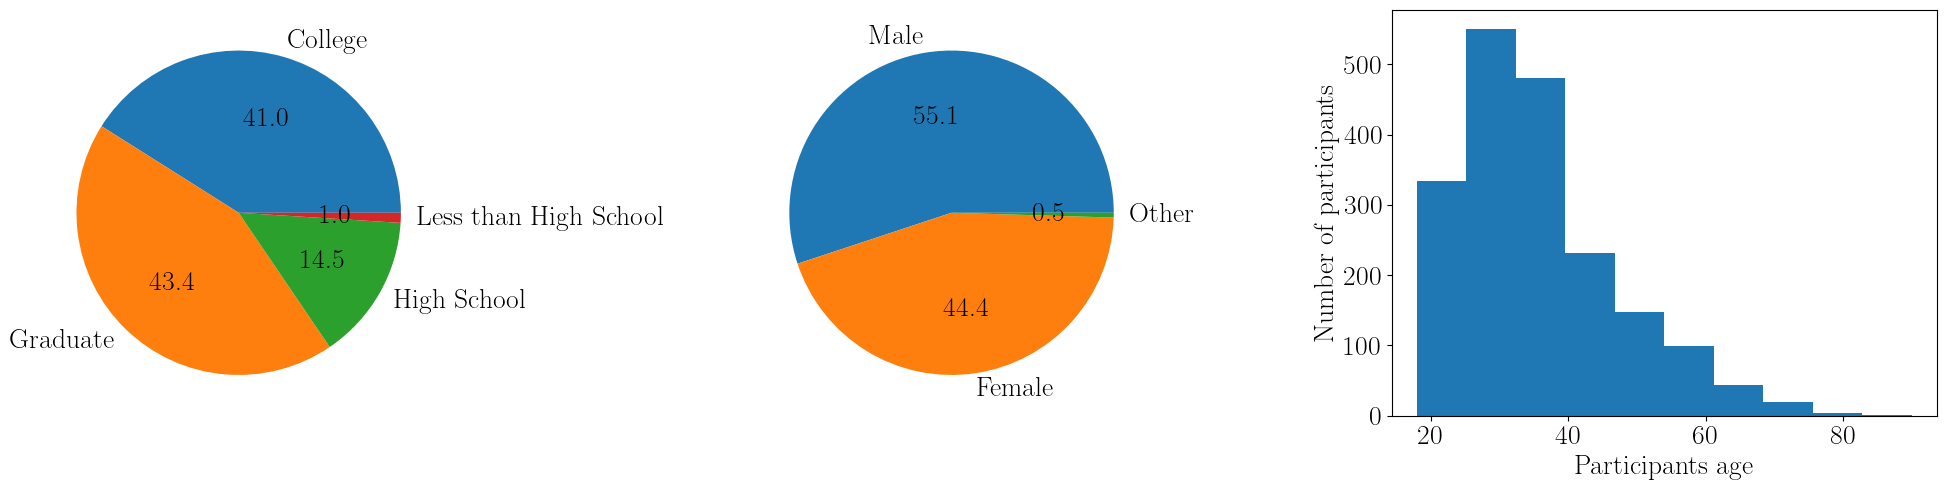
\includegraphics[width=15cm,height=4cm]{experiment/dists.png}
\caption{Distribution of age (left), gender (middle) and education (right) of participants. \gb{fix plot. colors, ratios. gender: probably a pie chart. axis labels + gaps + ordering on education}
}\label{fig:distribution}
\end{center}
\end{figure}

The small elections (\textsc{Small-A} and  \textsc{Small-B}) consist of 10 candidate projects while the larger elections  (\textsc{Large-A},  \textsc{Large-B}) have 20 projects, all with a budget of $500,000$.
Project descriptions and costs were taken from real participatory budgeting elections from across the world.  
Each project was assigned a location on a map of the  city  and categorized in one of five  categories   (education; streets and transportation; culture and community; facilities and recreation; environment, public health and safety). No project appeared in multiple elections.  
Full  details  on every election including the project titles, descriptions,  costs and locations appear in the appendix.

 \begin{figure*}[h]
\begin{center}
%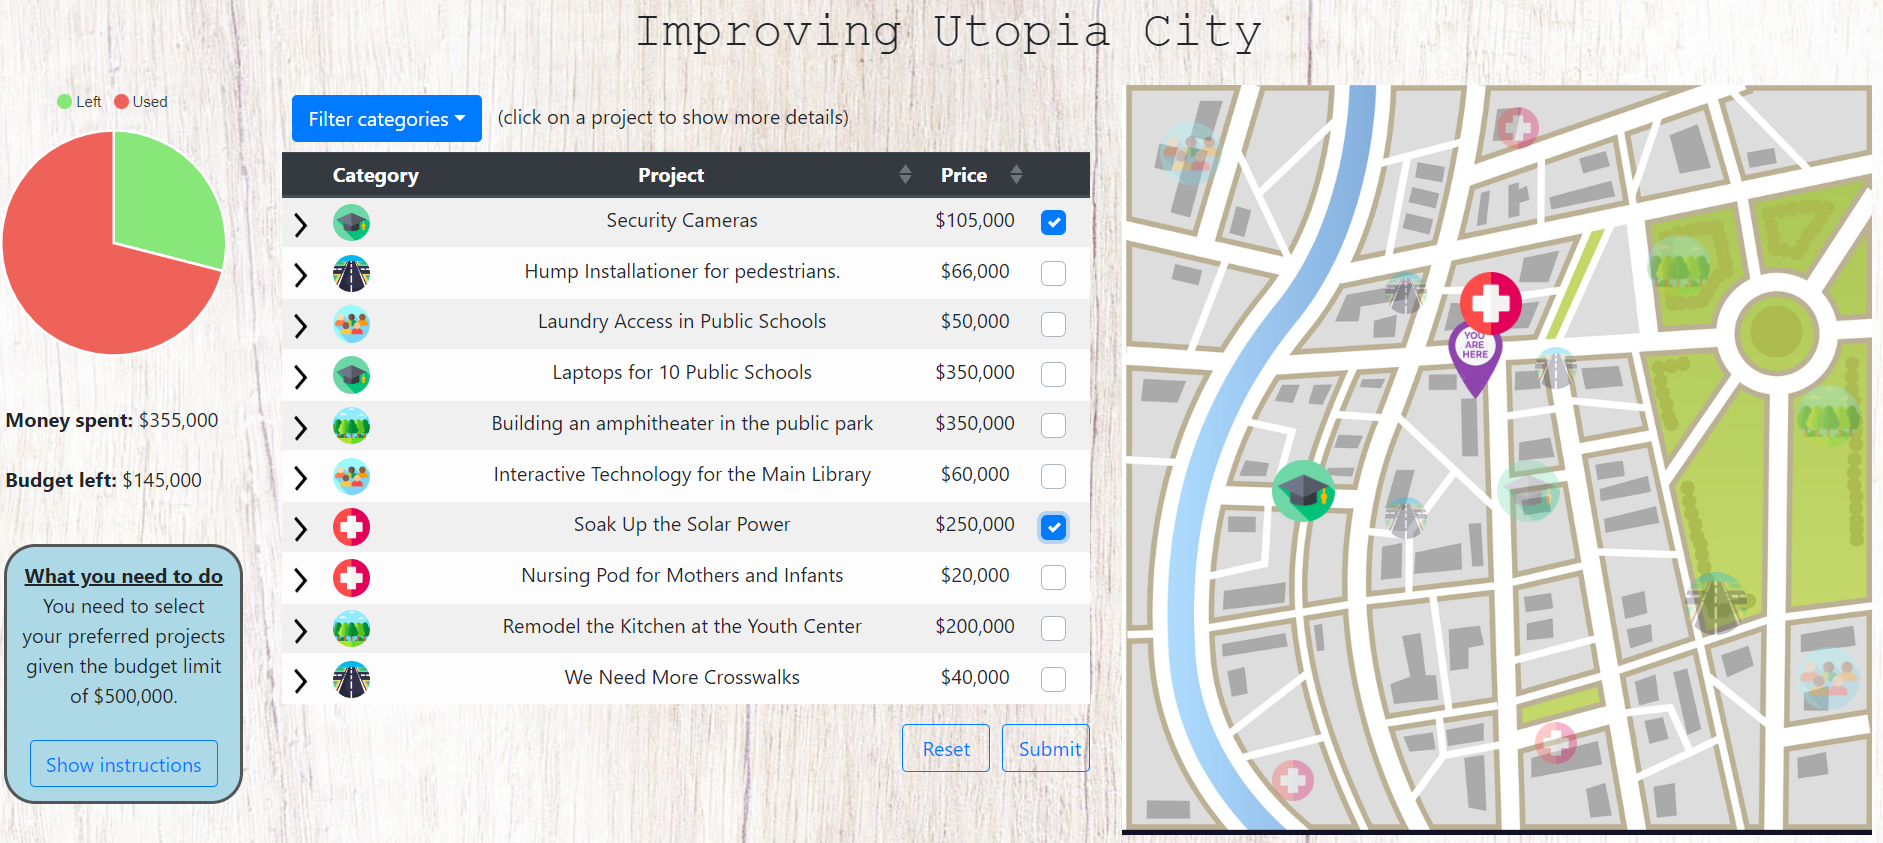
\includegraphics[clip, trim=0 3mm 0 0, width=15cm]{../experiment/full system.PNG}
\caption{The GUI shown to participants using the \knap{}  input format (center), showing  the city map (right) and budget (left).
}\label{fig:interface}
\end{center}
\end{figure*}
 
Participants were first presented with a written and video description of the PB voting task. They had to pass a simple quiz about the task in order to proceed. 
Next, participants carried out the voting task 
in their allocated PB configuration.
Each participant was assigned a  (random) location on the city map and   shown the description and location of the projects. 
We expected that a voter's location relative to  the project may affect their   preferences (e.g., people may prefer to vote for a library  close to their current location). 
  

 Figure~\ref{fig:interface} shows the interface  presented to participants who were asked to cast knapsack votes. 
 The left-most column shows the instructions and an indication of what fraction of the budget remains to be allocated. The center column shows the category and title of each proposed project, and a participant can click on a project to see a more detailed description. The right-most panel shows a map of the city on which the locations of the voter and the projects are marked (hovering over a project highlights its location). The other interfaces used in the study may be viewed in the full version. Project costs was only displayed for \points{} and \vfm{}, where it is needed to form a vote. 
 
 After   submitting their PB vote, participants were required to answer several consistency questions about their vote that were  designed to identify voters who vote randomly or carelessly (exact questions can be found in the full version).  Finally, participants were asked to complete a short survey about their subjective experience of voting in the assigned format. They were asked to rate (on a scale of 1 to 5) how easy they found the task, how much they liked the user interface,   how   expressive  they found the input format,  and how much the project categories and their location on the map    affected their decisions (exact questions can be found in the full version). 
 
 Participants were rewarded a  fixed sum    for participation and  received a 75\% bonus for passing the  consistency questions. 
 IRB approval was obtained from the corresponding institution. 

 
%%%%%%%%%%%%%%%%%%%%%%%%%%%%%%%%%%%%%%%%%%%%%%%%%%%%%%%

\subsection{Effect of Input Format on Voter Experience} 

 
We investigate the practical effects of using different input formats by comparing  the experiences of voters using the respective input formats.

This comparison has several components. Objectively, we record the time that it takes a voter to complete each of the first three stages of the task (completing the tutorial, answering the post-tutorial quiz, and casting a vote).  
We also report the number  of participants who fail the post-task consistency test and argue that a participant's inability  to recall simple information about the vote they just cast is correlated with the participant finding the task taxing, confusing or tiresome. 
More subjectively, we examine participants' self-reported scores from the post-completion survey.  

\subsubsection{Response Time}
The time it takes to complete a task is a recognized  proxy for  the cognitive burden  or difficulty of the task  \cite{rauterberg1992method}.  
%
The average time to complete each stage of the experiment is visually represented in  Figure~\ref{fig:time}.  Results in this section are averaged across elections and the conclusions do not change when looking at any individual election. %\gb{May be worth just looking at times for large vs small to see if there is anything interesting}

Participants voting in  the \vfm{}   format are consistently slowest to complete each stage of the experiment, suggesting that voters find \vfm{}  very hard to use. Based on the time it takes to cast a vote,  \points{} and \tapp{} are the next hardest formats to use. In the former case, we believe this supports the idea that asking voters for cardinal utilities is generally not feasible; in the latter, it  highlights the complications that sprout from  \tapp{} requiring cross-voter normalization  (as well as the fact that \tapp{} is a relatively niche format which voters are unlikely to have encountered before).  

Voters found \kapp{} the easiest to use, followed by \knap{} and \rank{}.

\begin{figure}[!h]
\begin{center}
%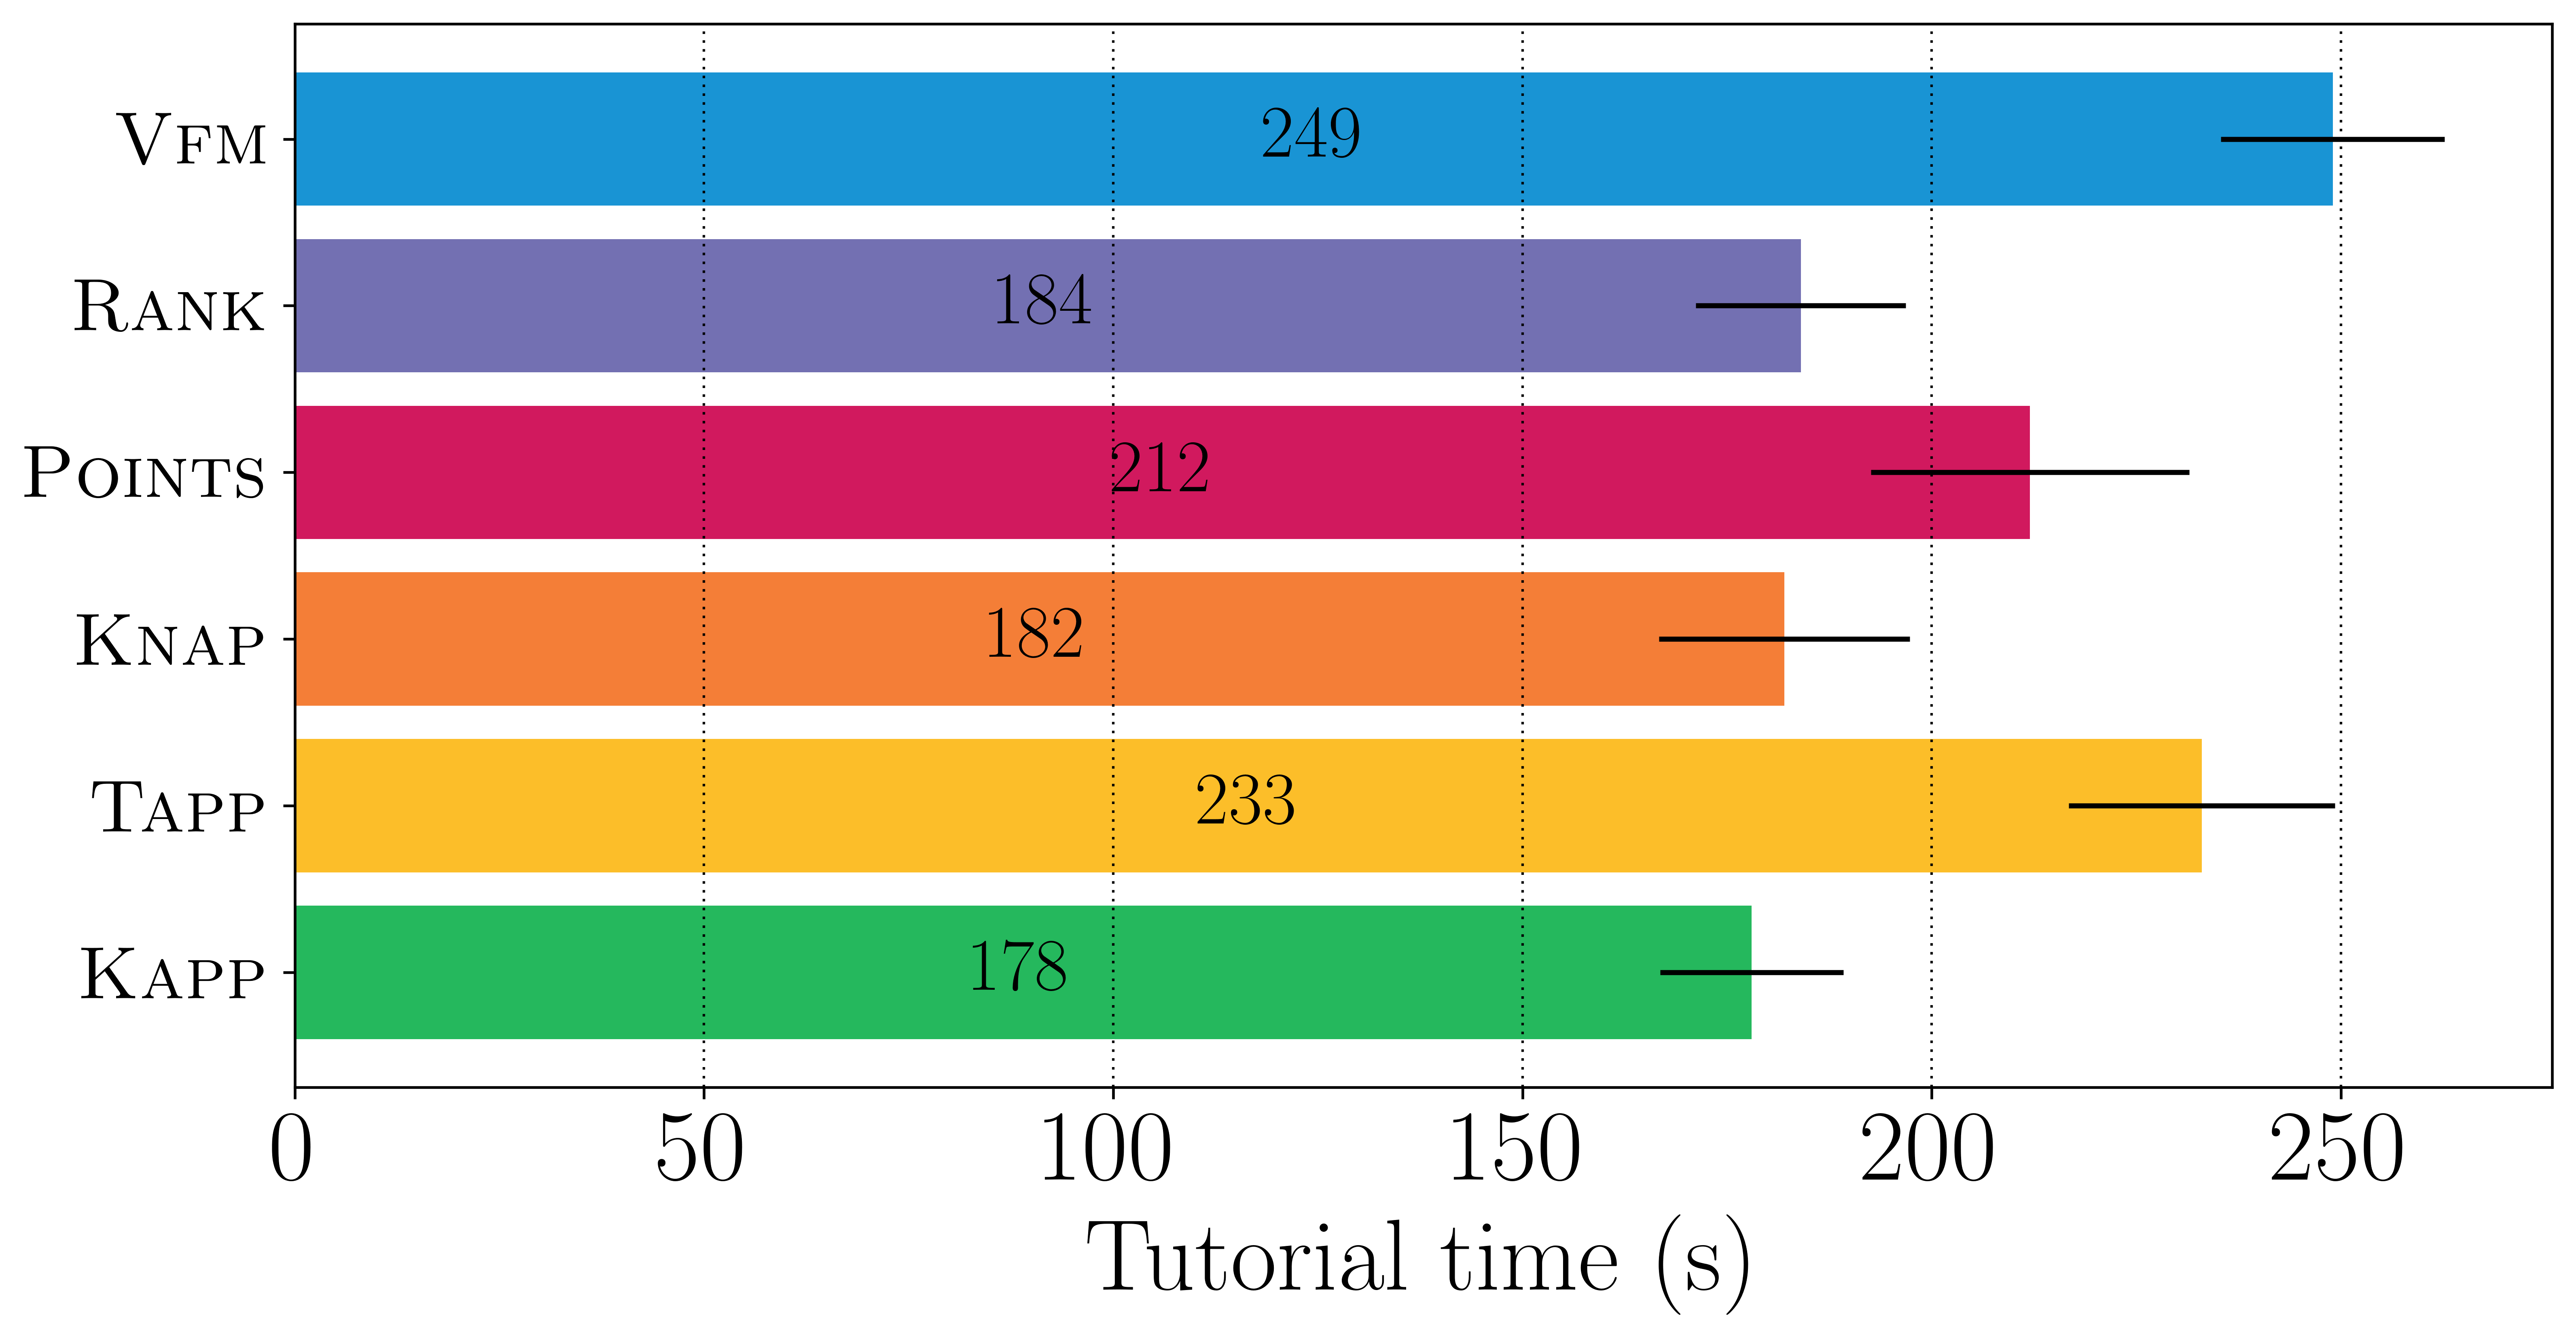
\includegraphics[width=5cm,height=4cm]{../experiment/tutorial_time.png}
%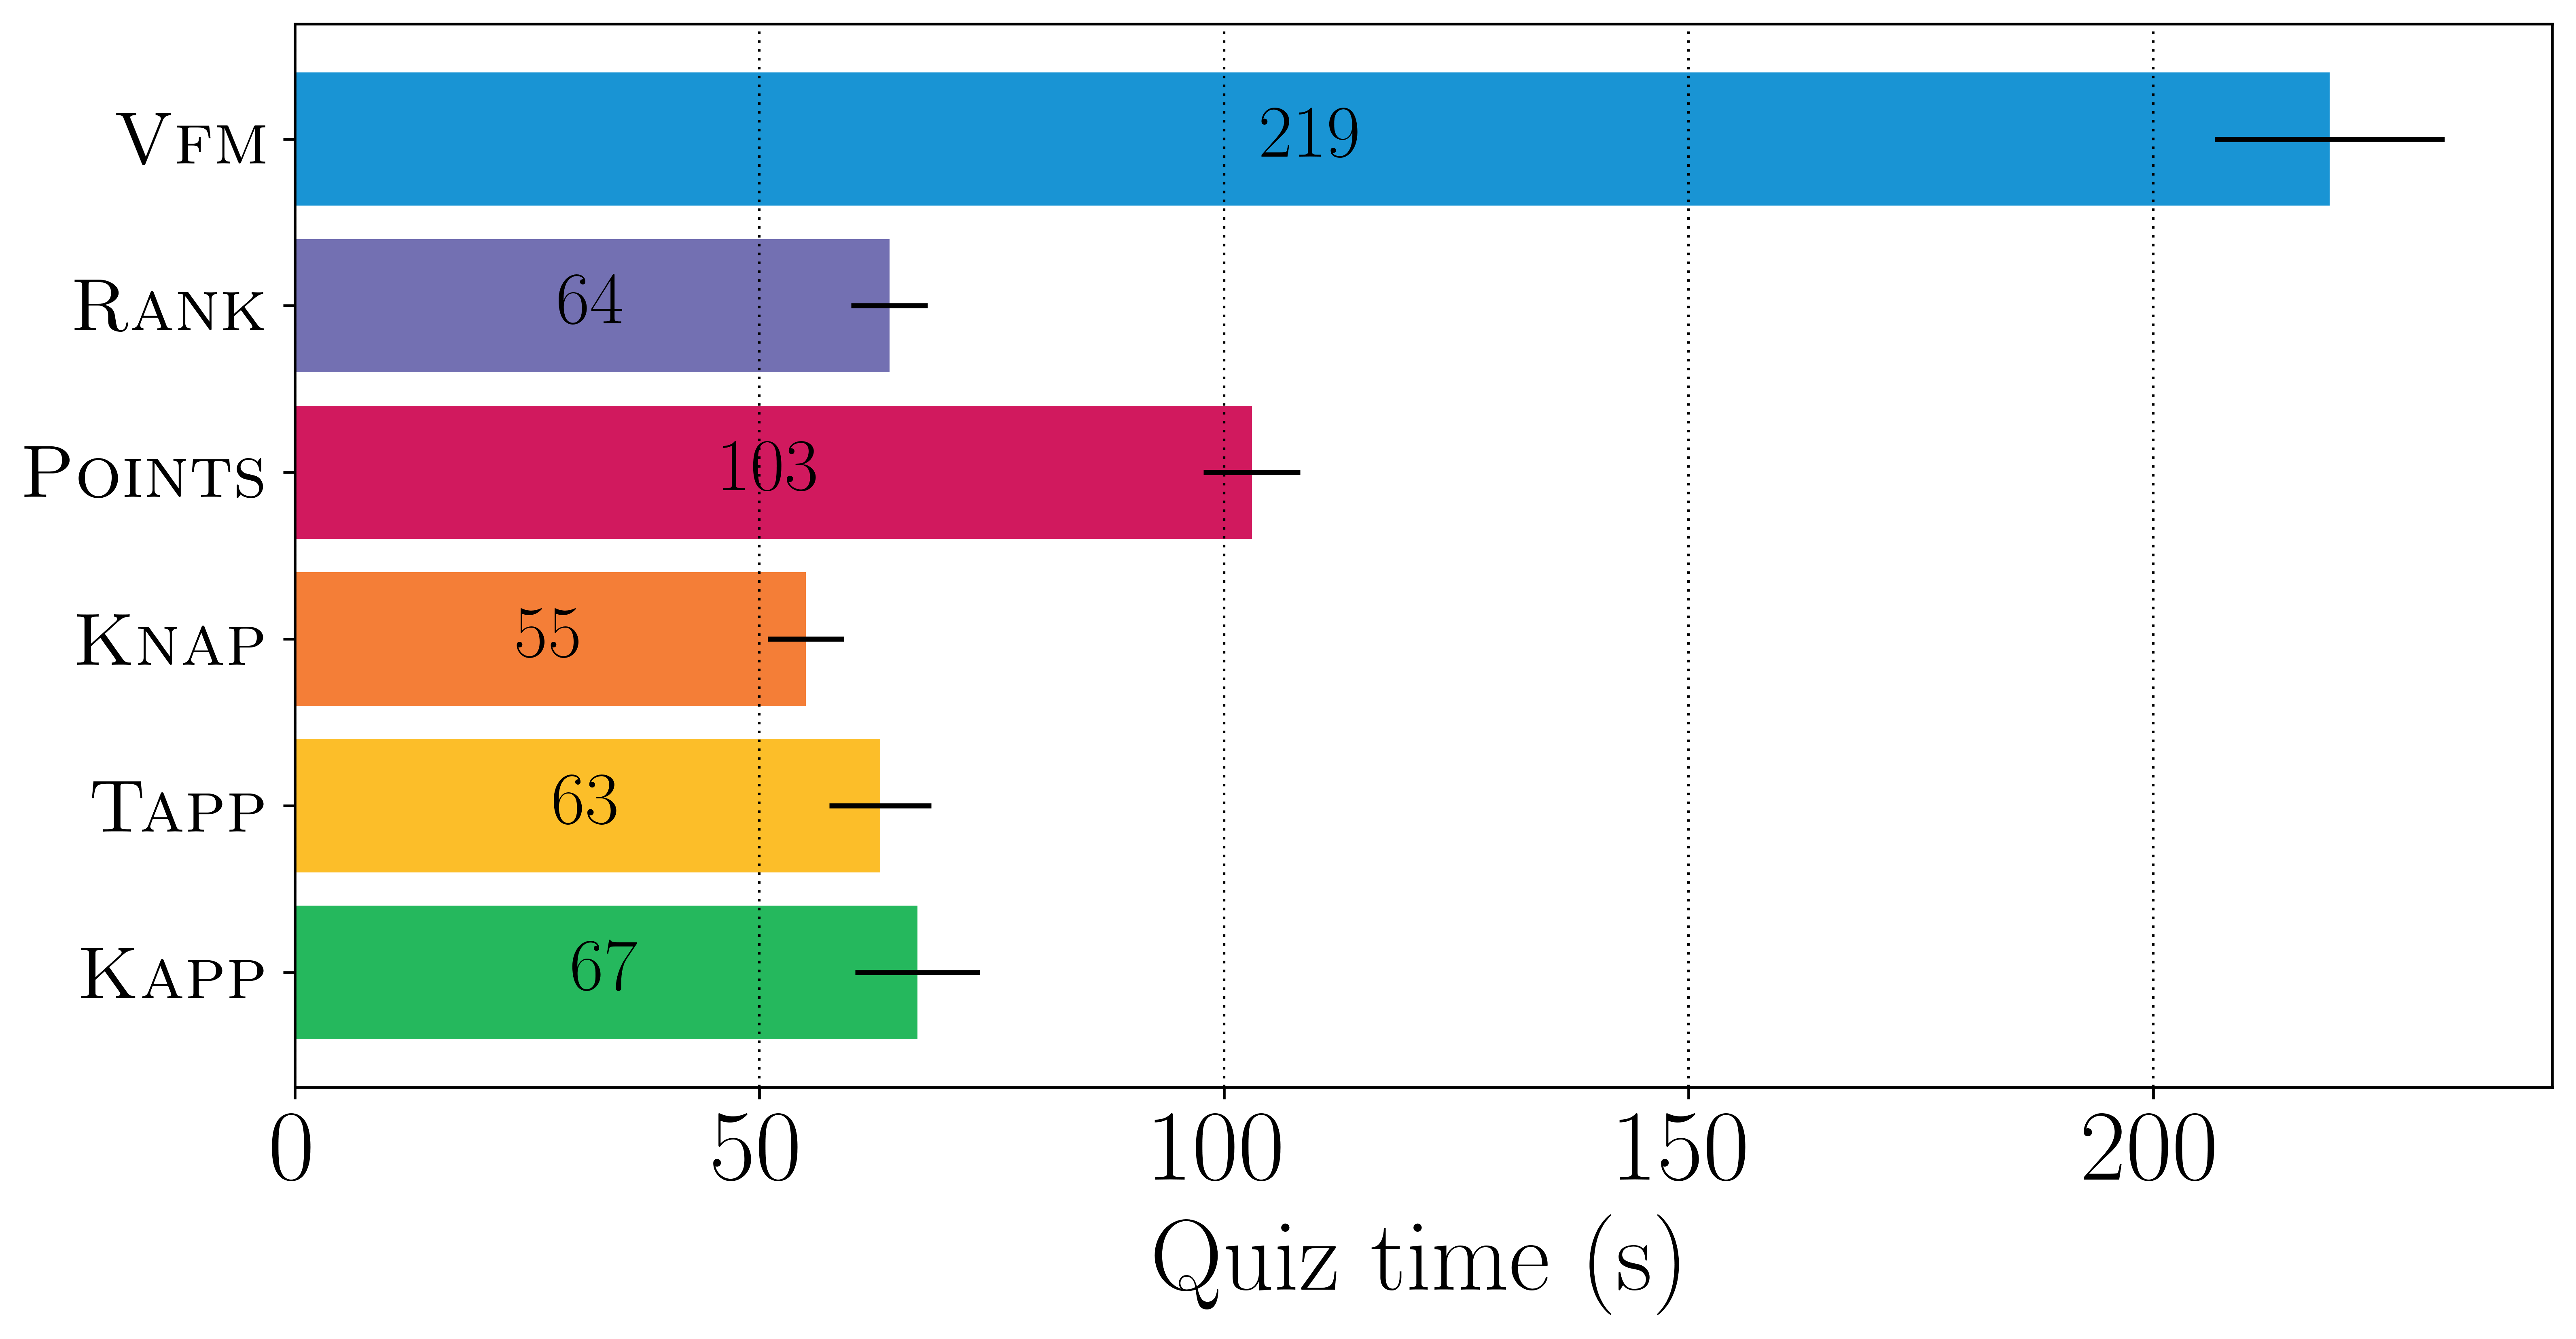
\includegraphics[width=5cm,height=4cm]{../experiment/quiz_time.png}
%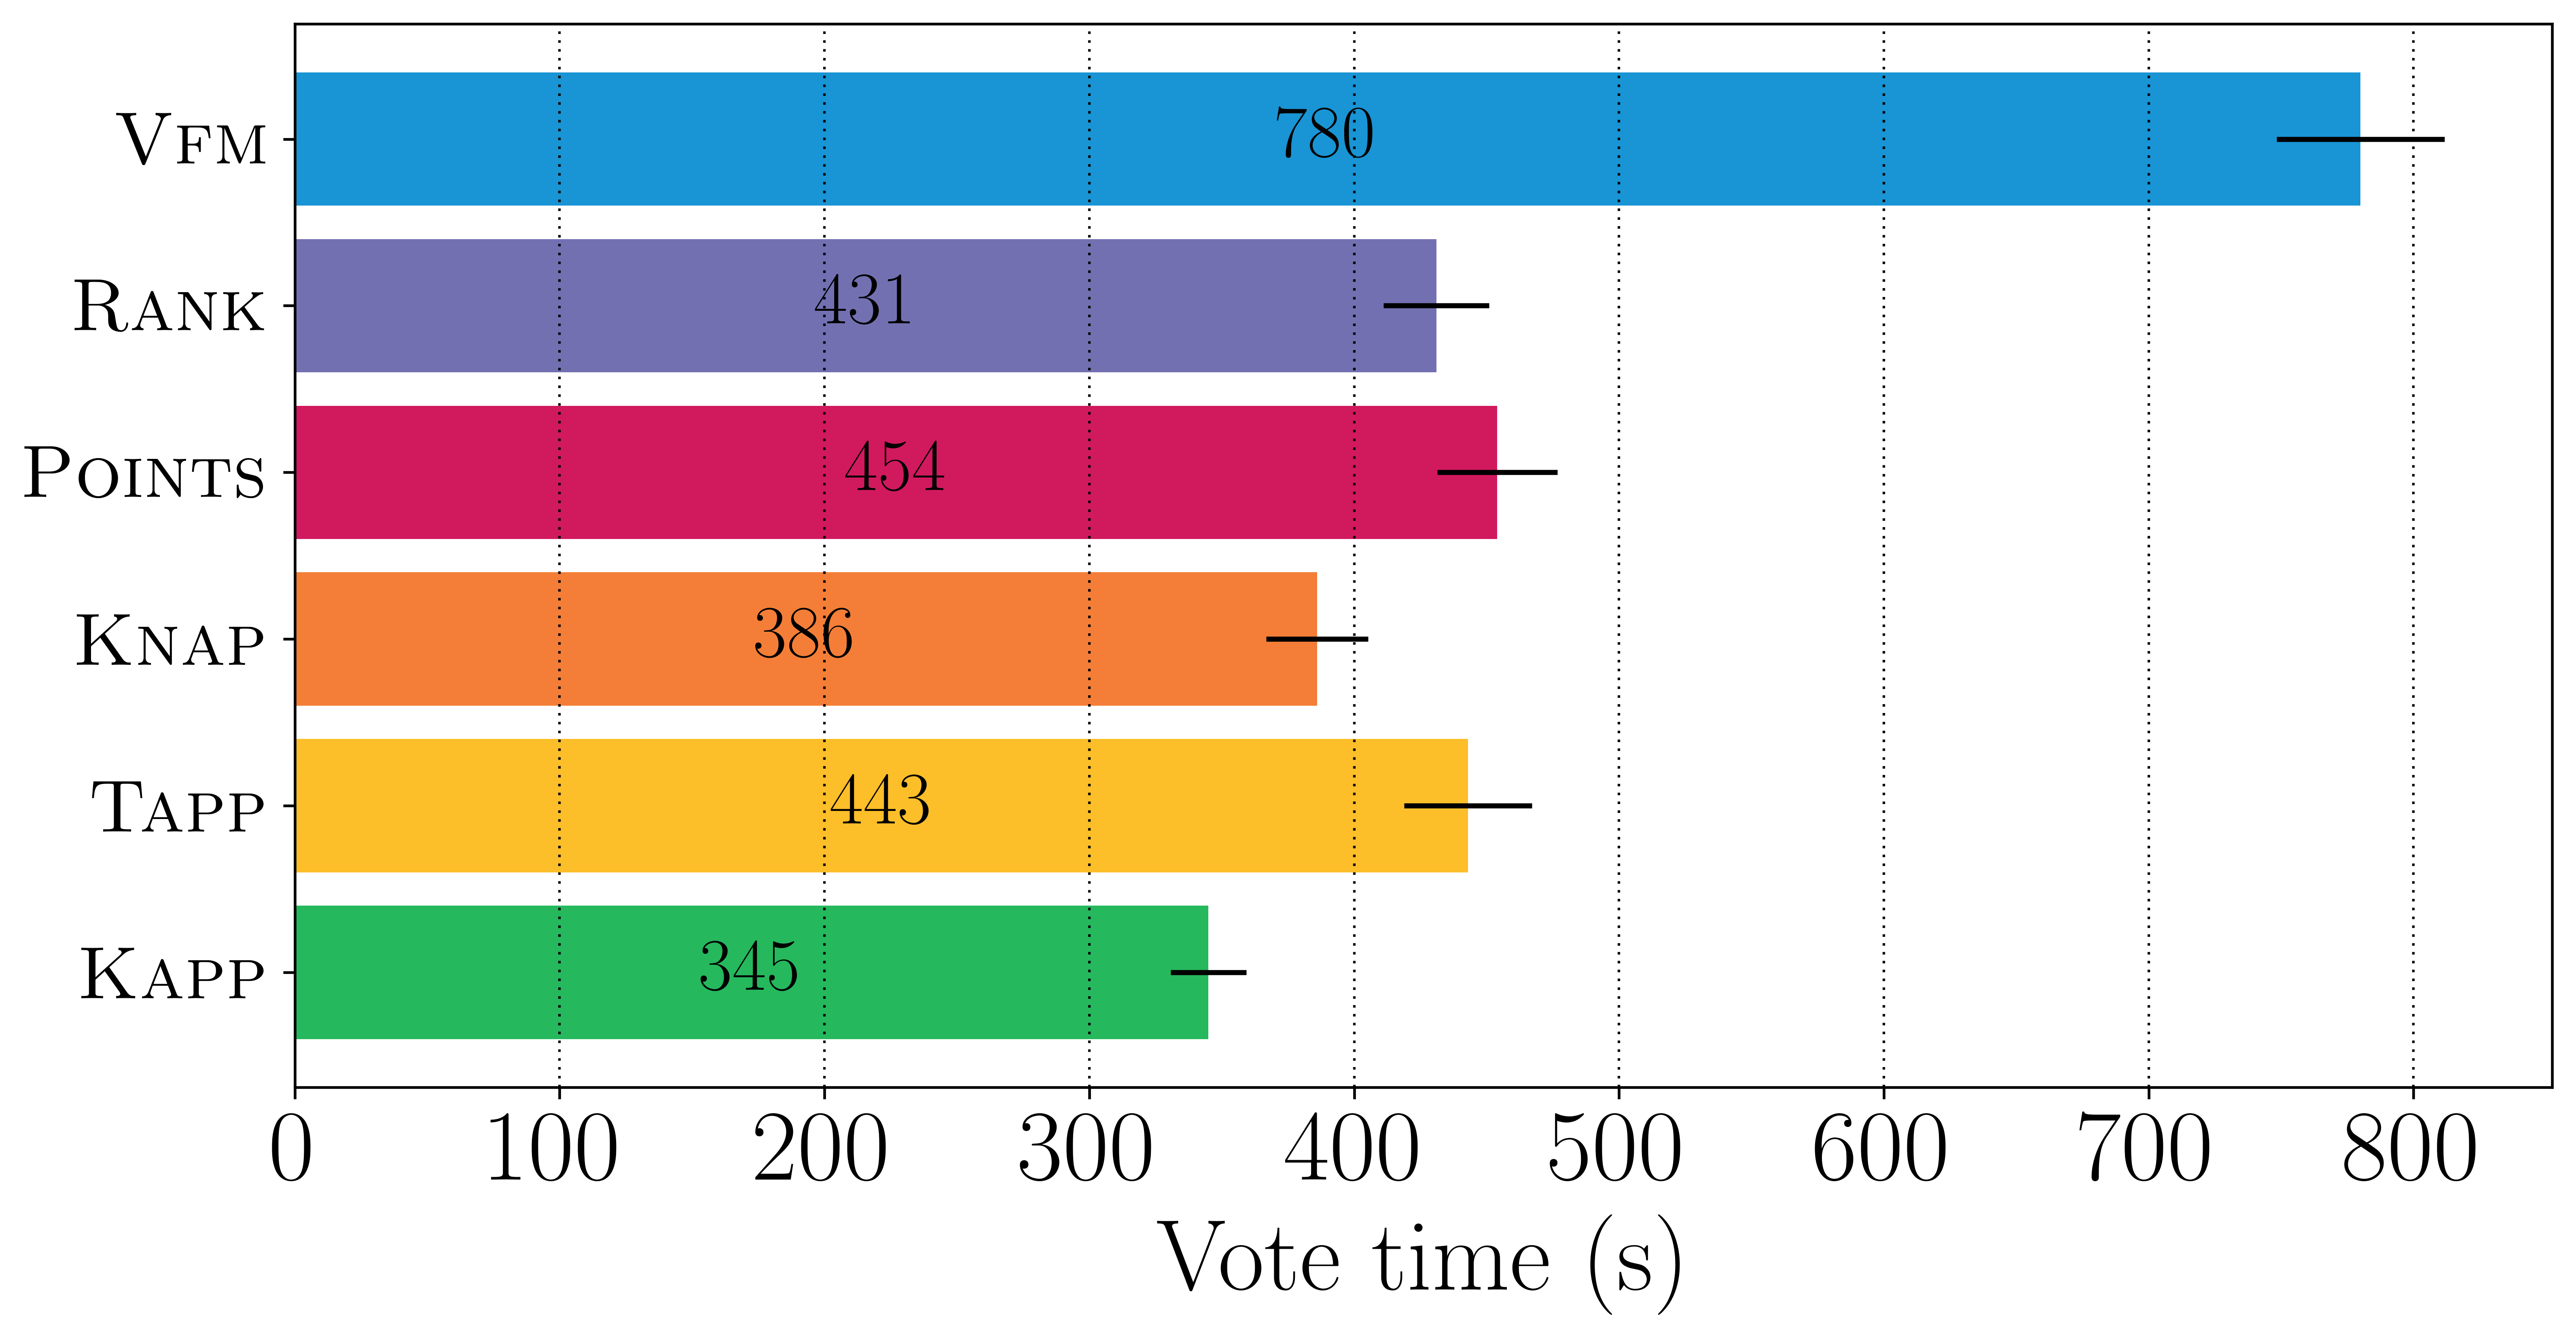
\includegraphics[width=5cm,height=4cm]{../experiment/vote_time.png}
\caption{Average time ($s$) to complete each stage. \gb{fix ratios, increase fonts}
}\label{fig:time}
\end{center}
\end{figure}

\subsubsection{Consistency Checks}
 
Of the roughly 75 participants  recruited for each of the 24 configurations of the experiment, on average 58 passed the consistency test. 

The consistency test  is designed to check whether the participant can recall simple information about the recently completed task. 
%
There are several reasons why a voter may fail the test. For example, they may answer randomly in order to complete task quickly,  become  distracted  if the task is too tiresome, or confused if the input format is hard to understand. As such, we  treat this as another signal about the difficulty of expressing  preferences in a given format. 

 

We  compare the rate of passing the consistency test across input formats. 
Participants using the ranking-based formats were most consistent, followed by the approval-based formats.  We speculate that the high consistency of \vfm{} is, at least in part, thanks to the inordinately long amount of time voters spend considering their votes. Users of \points{} were comfortably the least consistent, which  supports earlier evidence that providing cardinal utilities is a challenging task.

There was virtually no variation in the rate of passing the consistency test across the four elections. A complete breakdown of the results may be found in the full version. 

 

\subsubsection{Self-Reported Voting Experience}
In addition to the time it took participants to complete the task and how much they could recall about their submitted preferences, we also expressly asked them to rate various aspects of the experience on a scale of 1 to 5. 
Survey results are summarised in  Figures~\ref{fig:feedback} and \ref{fig:cat_map}. 
Results for the questions omitted from this discussion may be found in the full version.
In order to find statistical significance, we first used Kruskal–Wallis test to show the input formats give different results, followed by the Dunn test for post hoc comparison.
All of the survey questions   gave $p < 0.004$  for the Kruskal test. The Dunn test evaluated statistically significance   at the $p < 0.05$ level.



\textbf{Ease of use}  We asked the voters how easy they found the voting task. Unsurprisingly, participants found \vfm{} significantly harder to use than any other format. \points{} was rated as quite easy to use despite being one of the more time-intensive formats. \kapp{} was rated as significantly easier to use than all other  formats except \points. 



\textbf{Perceived expressiveness} We asked the participants how well they felt their vote captured their preferences. 
Participants found \kapp{} to be most expressive and, in particular,  significantly more expressive than  \tapp, \vfm, and \points. It is somewhat surprising that \kapp{} was rated as more expressive than \points, since you can infer a \kapp-vote from  your \points-vote; we speculate that the relative complexity of  \points{} explains part of this phenomenon. It is also possible that participants conflated expressiveness and ease of use, or failed to consider alternatives to the format presented to them.
\vfm{} was perceived to be least expressive by some margin. Again, the  difficulty of using \vfm{} and the fact that voters are forced to explicitly consider project costs may have contributed to the perception that it is less expressive than \rank, which also asks for a ranking of alternatives.  


\begin{figure}[!h]
\begin{center}
%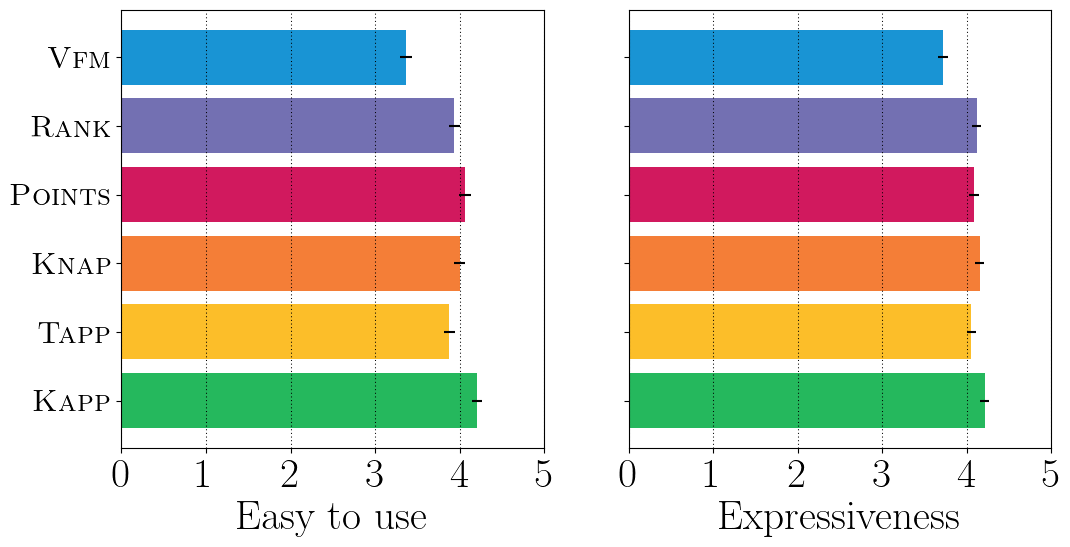
\includegraphics[width=8.5cm]{../experiment/survey1.png}
\caption{The average feedback for each input format.
}\label{fig:feedback}
\end{center}\vspace{-3mm}
\end{figure}

\begin{figure}[!h]
\begin{center}
%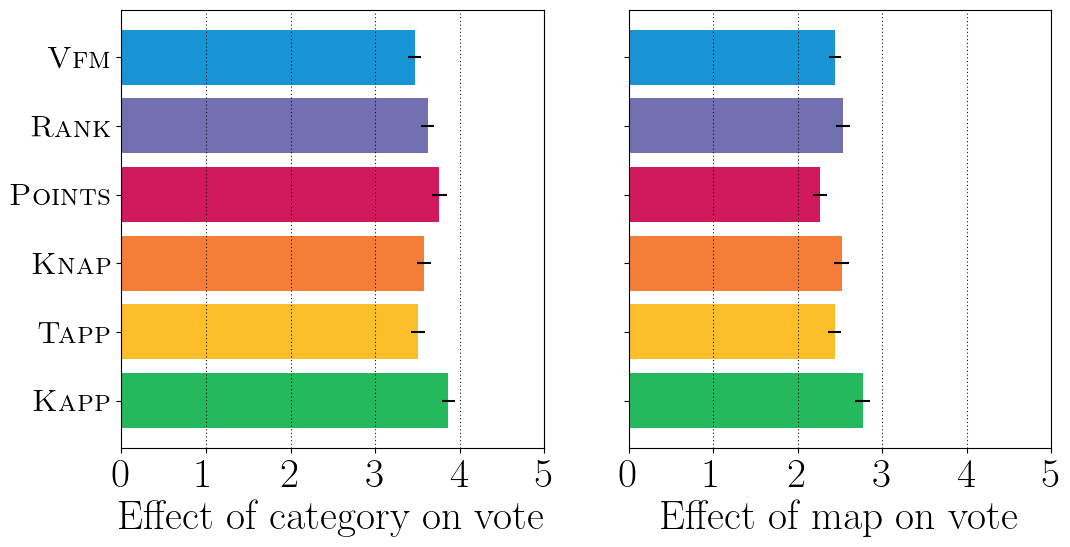
\includegraphics[width=8.5cm]{../experiment/survey2.png}
\caption{The average effect of the categories and the map.
}\label{fig:cat_map}
\end{center}\vspace{-5mm}
\end{figure}


\textbf{Effect of additional information}
Projects were assigned to one of five categories (e.g.\ transport or education) and given locations on a city map. Two survey questions asked about the extent that project categories and the map influenced participants' preferences. These results are summarised in Figure~\ref{fig:cat_map}.
%
Participants using \kapp{} were influenced  more by project locations than any other group. Similarly, \kapp-voters paid significantly more attention to project categories than all other groups except \points-voters. 
It may be that the \kapp{} format was easy enough to understand and use that it freed participants up to consider additional, non-core information about the projects and   election in their decisions. 


\subsection{Stability of aggregation methods}  
\label{sec:aggregation}
 %In  this section we  analyze the effect of aggregation methods  on the outcome of the elections.


 

%We   study the   stability of the different aggregation methods. 



In the first experiment, we repeatedly sample $n'=40$ participants per configuration  and aggregate the resulting vote profiles using greedy aggregation and \mes{}. This process is repeated 200 times.% (enough for convergence). 
%
The fraction of repetitions in which each project is funded in each configuration is summarized   in a heatmap in Figure~\ref{fig:heatmap} for binary utilities. The top row of results corresponds to greedy aggregation and the bottom row to \mes. Within each panel projects are ordered in order of increasing cost, and the cells range from white (meaning the project is never funded) to black (always funded). \gb{TODO:need a similar heatmap for 0-cost utilities. include that in discussion here or push to appendix with comment about similar results. }

\begin{figure*}[h]
\begin{center}
%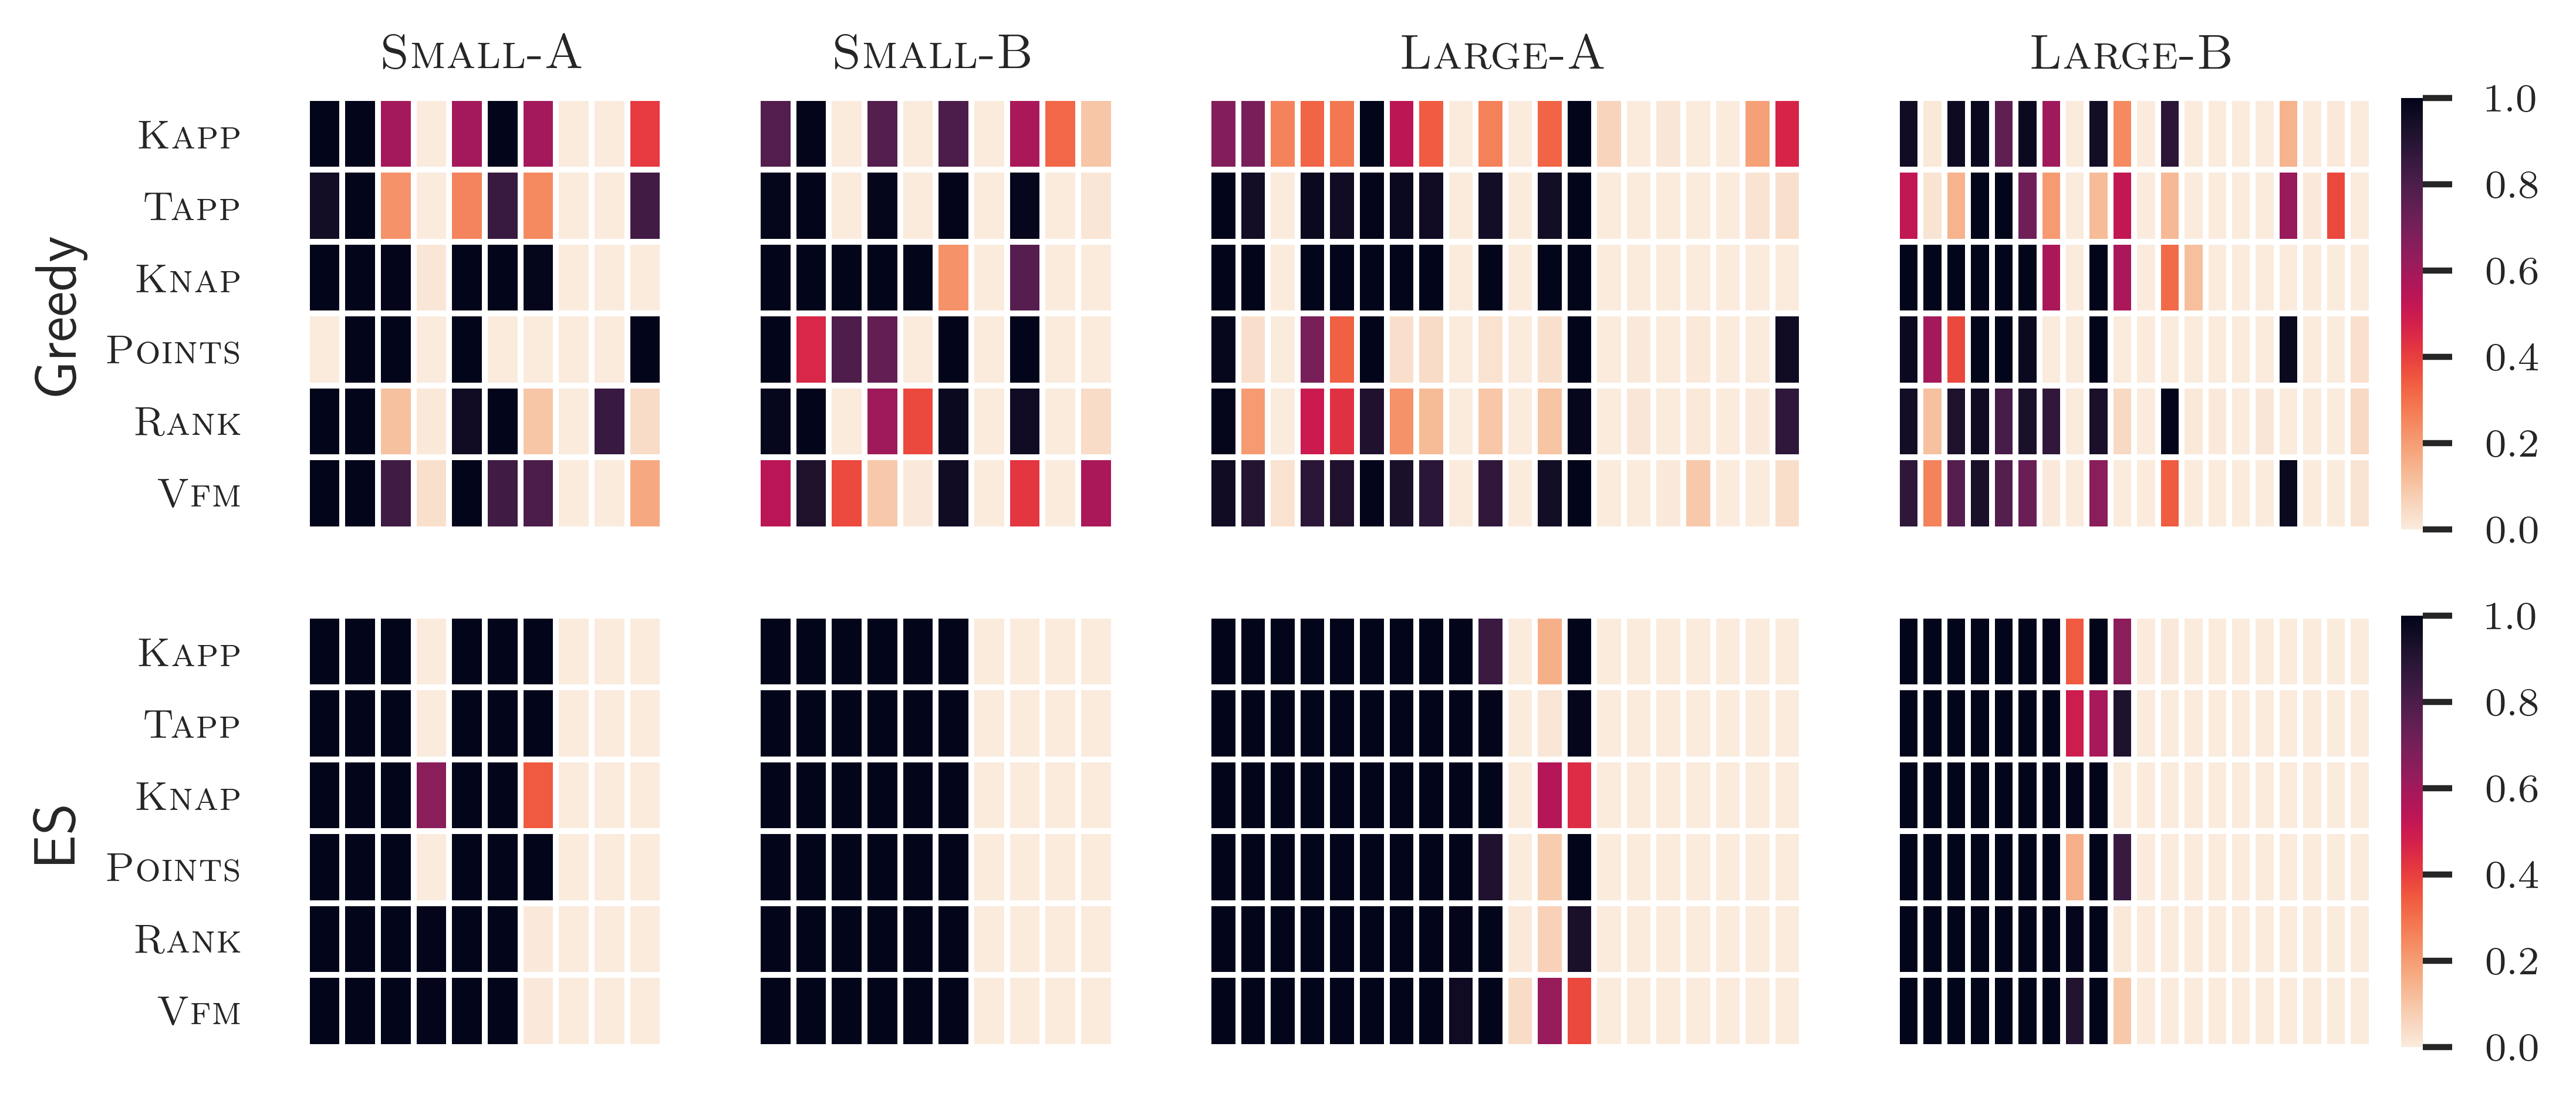
\includegraphics[width=15.5cm]{../experiment/heatmaps.png}
\caption{Stability heatmaps for  greedy aggregation (top) and \mes{} (bottom) with binary utilities in each election. 
Within each panel each row represents an   input format and each column a project (ordered in increasing cost).
 The intensity of a cell indicates the fraction of instances in which the project was funded. \gb{fix greedy/es}
}\label{fig:heatmap}
\end{center}\vspace{-3mm}
\end{figure*}

Strikingly, the outcome of the election is almost entirely unaffected by the choice of input format when using \mes{} --- the majority of the projects are either always funded under every input format or never under any. Greedy aggregation exhibits this property only in rare instances, for example, the outcome of \textsc{Large-A} does not change if the input format is changed from \knap{} to \tapp.  This robustness to the choice of input format remains present when the number of sampled voters is varied $n'\in\{10,20,30\}.$

We also observe in   Figure~\ref{fig:heatmap} that \mes{} is robust to partial participation: it is very rare that the decision to fund a project changes across repetitions when sampling voters at random, i.e.\ under a uniform model of voter participation/abstention. Greedy aggregation does not exhibit this property. 

Of course, since we are sampling 40 votes from (on average) 58 consistent voters the sampled profiles are correlated. We repeat the experiment, sampling $n'\in\{10,20,30\}$ voters each time, to investigate what happens when vote profiles are less correlated. 
%


Figure~\ref{fig:entropy} shows the entropy for election   \textsc{Small-A} across   input formats for greedy aggregation and  \mes{} aggregation when varying the degree of participation (i.e. the number of sampled voters). 
Unsurprisingly, the correlation between vote profiles decreases and entropy increases  as fewer voters are sampled. 
The entropy of \mes{} is consistently significantly lower than that of greedy aggregation across input formats. We conclude that \mes{} is significantly more robust to partial participation than greedy aggregation. One exception is worth highlighting, the entropy of greedy aggregation with \knap{} votes is fairly competitive with that of \mes. This suggests that if the organizers of a PB election are dead-set on using greedy aggregation and also worried about the effect of partial participation,  \knap{} may be an attractive option.  
%
For the other three elections,   \mes{} aggregation comfortably outperforms greedy aggregation across all input formats and sample sizes (except similar results for \knap{} in election \textsc{Large-A}). Full results  may be found in the full version. 



We conclude this section with an observation from  Figure~\ref{fig:heatmap} unrelated to stability. It appears to be the case that more expensive projects are rarely funded  when using \mes{}.  We believe this may (at least for the binary input formats)  be an artefact of assuming $v_i(p)\in \{0,1\}$, which makes it very hard for an expensive project to have a ratio of utility to cost that justifies funding it. It remains to be seen whether this trend persists, for example, when assuming $v_i(p)\in \{0,c(p)\}$. \gb{Todo: reword observation once we have both 0-1 and 0-cost. perhaps also include a large election here}

\begin{figure}[!h]
\begin{center}
%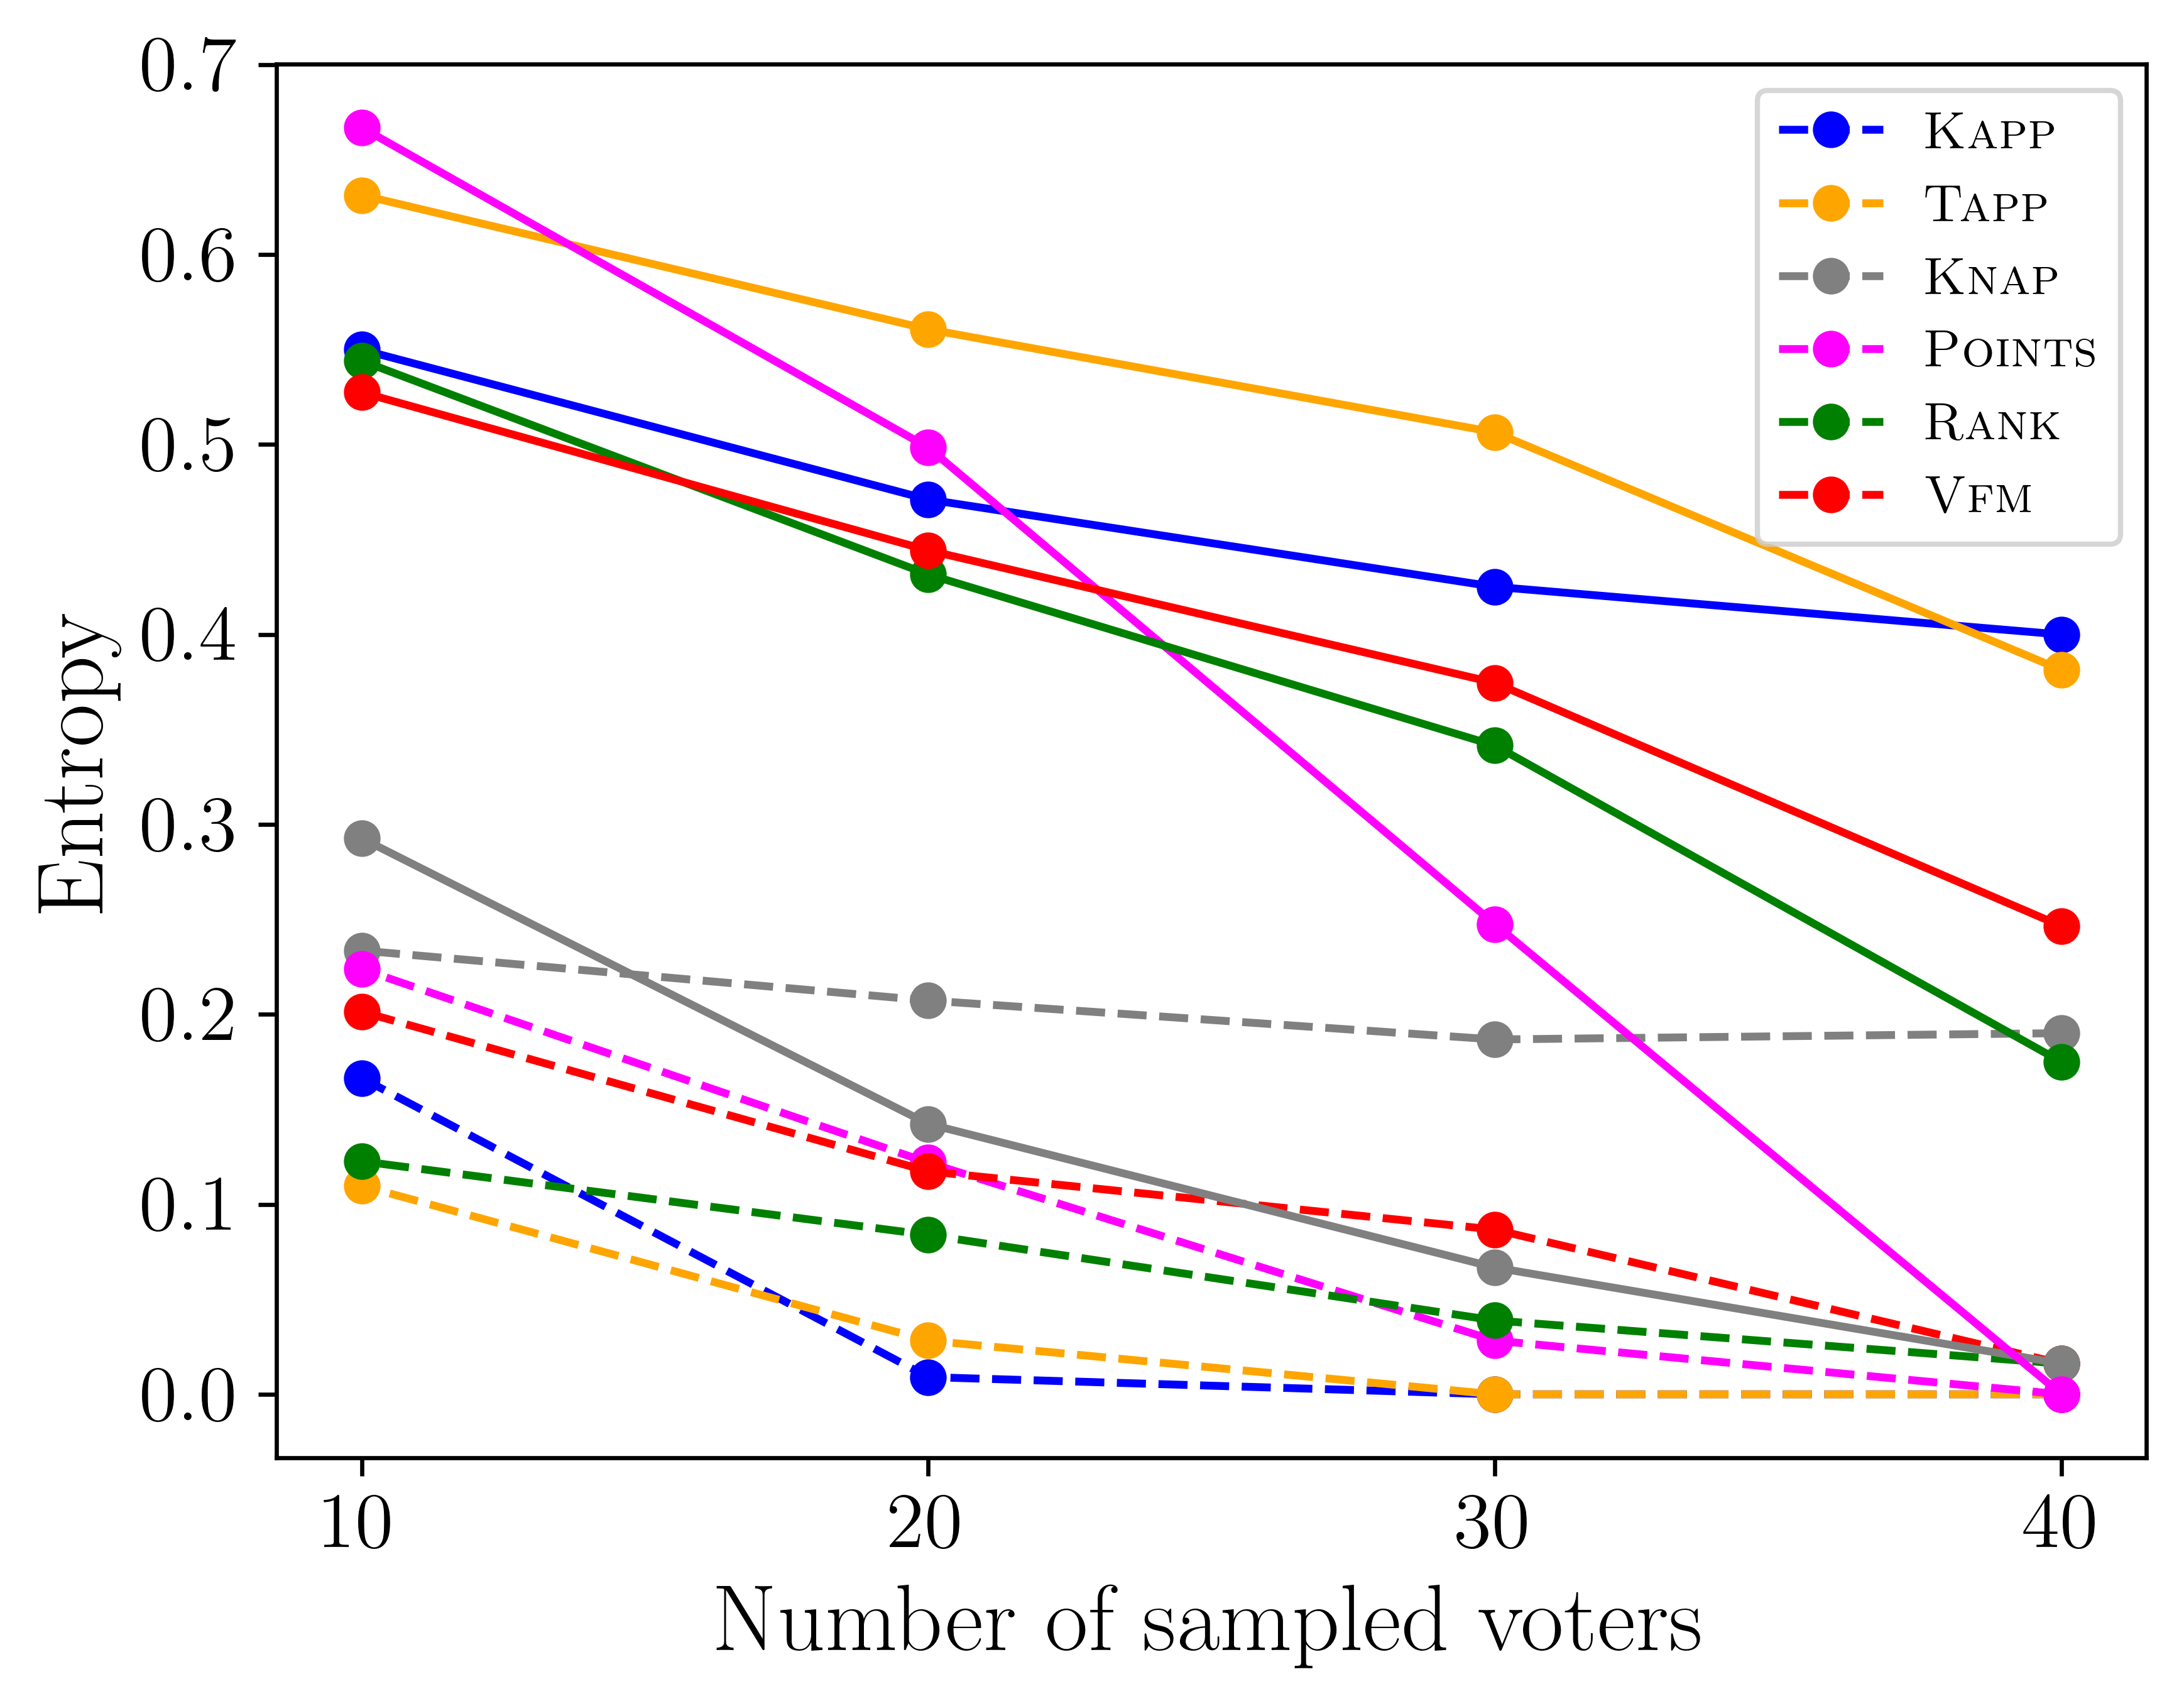
\includegraphics[width=7.5cm]{../experiment/entropy_small_a.png}
\caption{Entropy for each input format under  greedy aggregation  (solid lines) and \mes{} (dotted lines)  as the number of sampled voters changes. \gb{Todo: similar plot for 0-cost utilities}\rf{We need to think how to do this. Putting all 4 in a graph like this will make it unreadable I think}
}\label{fig:entropy}
\end{center}
\vspace{-3mm}
\end{figure}

% \subsection{Social Welfare}
% An obstacle to comparing outcomes based on social welfare is participants are assigned only one format, so there is no common basis of comparison when aggregating vote profiles from different formats. To address this, we make the assumption that, since voters are randomly assigned to input formats, the distribution of voter preferences are the same across formats. As such, we can deduce voter valuation functions from the full vote profile in \emph{any} format and treat these aggregated values as a proxy for the welfare of all voters, regardless which format they used.\footnote{ We caution that this is at best a very coarse evaluation, since assuming a value based on  a vote in any of the formats requires very strong assumptions. 
% } 

% We report in Figure~\ref{fig:welfare} the   social welfare (averaged over the four elections) as measured when treating the full profile of \points{} or \knap{} voters as representative. 

% Neither aggregation method strictly outperforms the other. However, we observe that, when using greedy aggregation, the choice of input format can have a large effect on welfare. This is seen most clearly when using \knap-voters to compute welfare. Unsurprisingly, \mes{} is less sensitive to  the choice of input format and   achieves very similar welfare across input formats.
% Results when using the other formats to measure welfare are less extreme than the results shown here and may be found in the full version.

\gb{responsiveness  message not entirely clear. perhaps in discussion  + point to appendix}

\section{Stability in real elections}\label{sec:stability}
% Pabulib instances
% \begin{itemize}
%     \item Overall plots, comparison with 4 lines. scatter plots with 
%     \item Plot with size on x axis - which instances
% \end{itemize}  

We extend our study of the stability of aggregation methods to participatory budgeting instances available on a public repository called \pabu{} \shortcite{pabulib}. \pabu{} consists of the votes cast in more than 700 participatory budgeting elections held across Poland. 
These real-world elections are much larger than those in our experiment, the largest elections have more than $100\,000$ voters and more than 100 projects.
In contrast to our experiments voters cast a vote in only one format; we focus our analysis on elections reporting approval votes between 2015 and 2022, of which there are   498. Of these, we omit xxx due to ....\gb{Roy   please check all these numbers to make sure we report what we actually did. }

We run a   similar experiment to before, sample an $n'$ fraction of voters from each election and aggregate these votes  using greedy aggregation and \mes, assuming both binary and cost utilities. This repeated XXTODO times, we report averaged results in \Cref{fig:pabulib:stability} for $n'\in \{0.01, 0.03, \ldots, 0.11\}$.\footnote{Constraints on computation time are the only obstacle to further experiments: the experiment for $n' = 0.11$ takes roughly xxx to complete. }
We analyze elections with at most 10 projects separately from larger elections. 

\begin{figure}[!h]
\begin{center}
%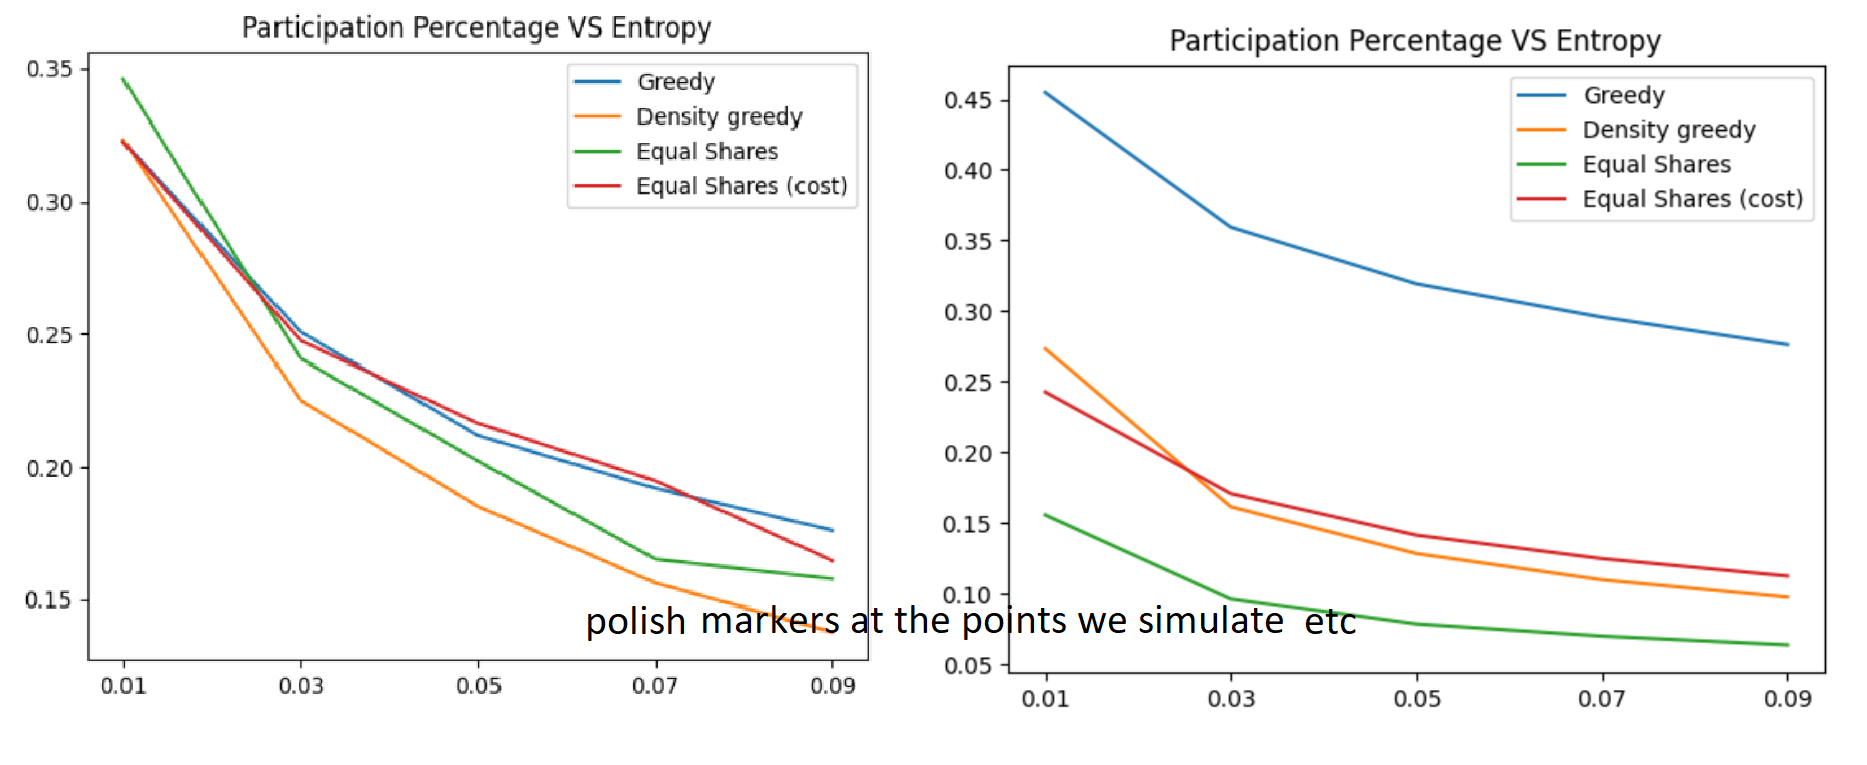
\includegraphics[width=14cm]{../experiment/tmp-stability1}
\caption{Entropy for each input format  and aggregation rule under binary and cost utilities. Results for small instances of at most 10  projects are left, larger instances right.  
}\label{fig:pabulib:stability}
\end{center}
\vspace{-3mm}
\end{figure}

We observe essentially no difference in stability on small elections. However, \mes{} is considerably more stable than greedy aggregation on larger elections under both binary and cost utilities. 


Digging deeper into what exactly causes the difference in stability trends between small and large elections, we define the difference in entropies 
\[
\Delta(A) = \text{entropy}^{\mes}( A) -  \text{entropy}^{Greedy}( A)
\]
on instance $A$.\footnote{All the \pabu{} instances we analyze consist of approval votes, so we suppress the dependence on $V$, the voting format.} 
Let $B_A$ and $\bar{c}_A$ be the budget and average cost of a project in instance $A$. 
\Cref{fig:pabulib:entvsbudget} plots  $\Delta(A)$ against the expected number of projects funded, $n_A \triangleq B_A / \bar{c}_A$ for the  \pabu{} instances with at least 10 projects under 10\% participation.
Strikingly, greedy aggregation has lower entropy than \mes{} almost exclusively on those instances where the budget and project costs are such that at most two projects can be funded. On instance with more flexibility and a larger number of feasible outcomes, \mes{}  is more stable. These findings hold when varying the utility model (see \Cref{fig:pabulib:entvsbudget}, right) and the fraction of votes sampled (refer to the appendix). 


\begin{figure}[!h]
\begin{center}
%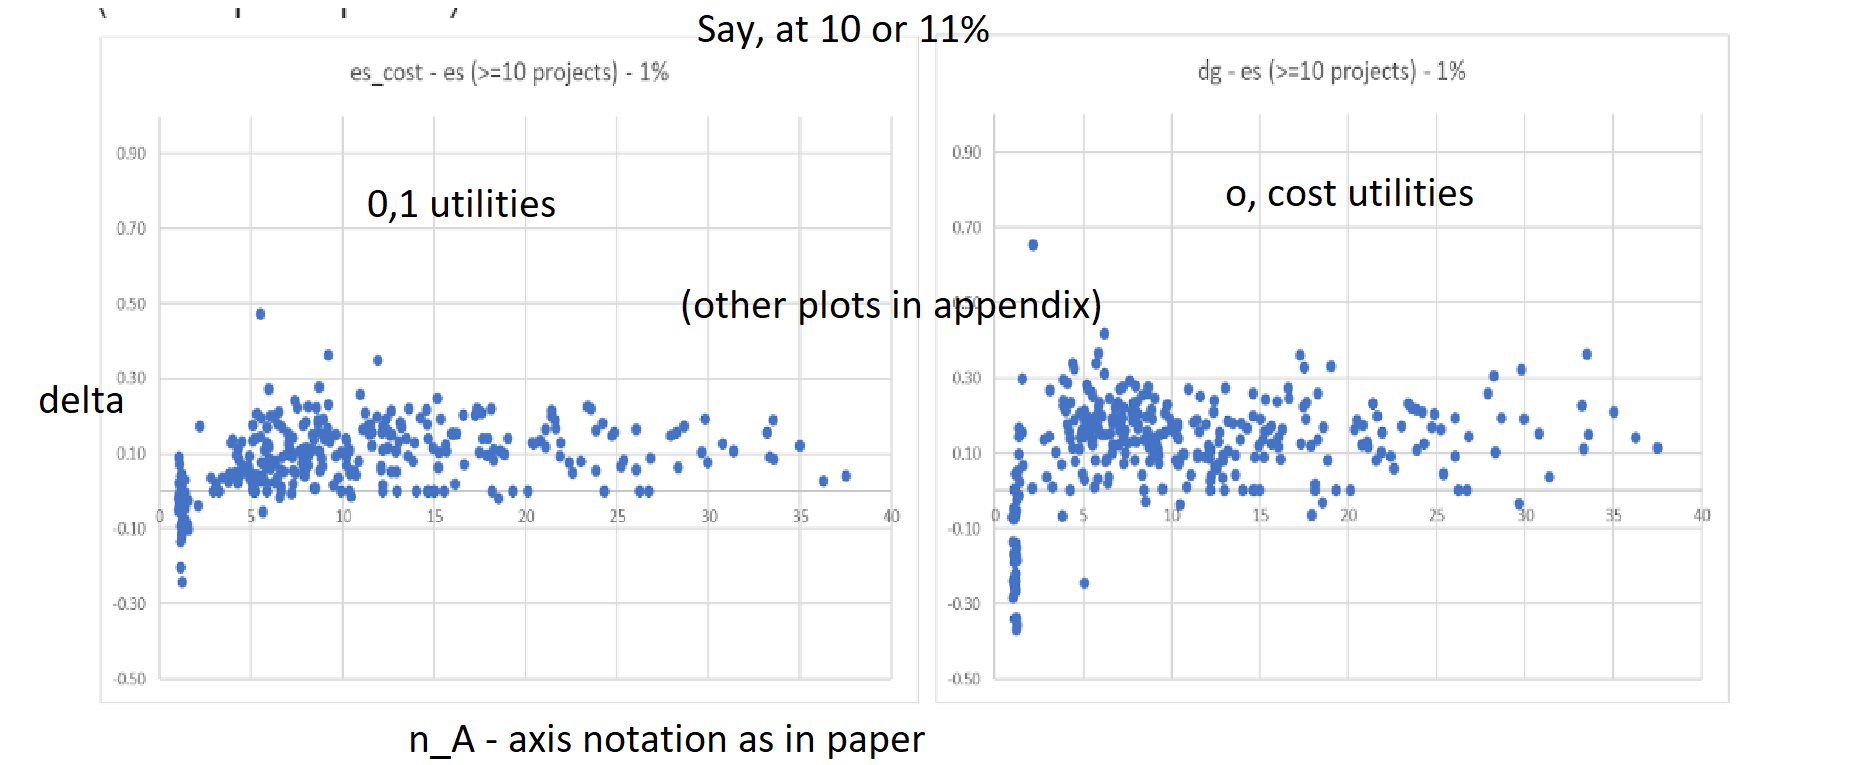
\includegraphics[width=14cm]{../experiment/tmp-stability2}
\caption{Difference in entropy between \mes{} and greedy at 10\% participation versus the average number of projects funded across large instances for binary utilities (left) and cost utilities (right).   
}\label{fig:pabulib:entvsbudget}
\end{center}
\vspace{-3mm}
\end{figure}


\section{Discussion} 
These results highlight practical insights  for the design of real participatory budgeting elections. 
When choosing an input format, we find no reason to deviate from the current standard practice of  using \kapp{} voting: Voters find the format easy to understand, easy to  use, and believe it allows them to express their preferences accurately. 

Greedy aggregation is used almost universally,  however, our experiments find that \mes{} has  two  big advantages over greedy aggregation.  First,  the outcomes are largely stable and unchanged when only a subset of the population participates. In light of low levels of real-world participation, we believe this is a particularly attractive property. Second, \mes{} appears to be robust to the choice of input format, in other words, it affords the city officials responsible for administering the participatory budgeting election a great deal of freedom to choose an input format which meets whatever secondary objectives are deemed to be important. % means that it allows officials a large degree of freedom to choose an input format which suits their objectives

%One argument that remains in favour of greedy aggregation is its transparency: it is arguably easier to explain to voters than \mes{}. If greedy aggregation is used    and stability to partial participation is a primary concern, then \knap{} emerges as a fairly user-friendly format overall and a clear front-runner in terms of stability.


%\gb{Robustness as argument against stability. appendix. also social welfare - appendix. }

These recommendations should be taken in the context of the limitations of this study. First, the  behavior and preferences of participants recruited on Amazon Mechanical Turk may not be sufficiently similar to those of real voters.  Though we attempt to  ensure the findings are robust across the parameters of different elections by varying the number and type of projects, there is no mimicking the richness, variety and local idiosyncrasies of real-world instances. Similarly, real voter utilities likely exhibit complementarities and externalities  --- a far cry from our utility proxies. It is possible that, despite our best efforts, the   voter experience   was affected by the interface design choices we made. 

 We find find the argument for stability (extremely low real-world turnout) compelling, but it is certainly not the last word. An argument against stability is that an aggregation rule should be responsive;  the outcome of an election \emph{should} change when the preferences of the voters change.  An example of a well-publicized electoral process which is not responsive is gerrymandered congressional districts in the US, where voters are grouped in such a way that the elected representatives have are largely unaffected by swings in partisan support. Towards this line of thought we report in the appendix  on experiments aimed at responsiveness: we measure how many copies of each voter is required (how many similar voters they must recruit) to improve their utility from the funded set of projects. 
 This measure of responsiveness is largely inverse to stability but not strictly so, for example, with binary utilities \mes{} is both more responsive and more stable than greedy aggregation. 

We conclude with  two directions for future study.  
When it comes to designing participatory budgeting elections, the proof, to a large extent, should be in the pudding.   
One can imagine a  variant of the experiment presented in this paper in which votes from different PB designs are aggregated and voters are directly asked to compare different elections and outcomes on the transparency of the process, personal satisfaction, perceived fairness of the outcome, etc. 
Directly asking people their opinion about PB outcomes may yield new  insights   that can help inform design decisions while avoiding assumptions like  additive utilities. 

Democratic innovations live and die by the extent to which voters' voices are heard. But this requires representative participation. 
As a fledgling part of the democratic process, participatory budgeting appears to be particularly susceptible to poor participation. It is important to understand how   design choices around voting formats and the transparency of aggregation rules affects the participation (now and in the future) of voters from a wide range of socio-economic backgrounds. Our stability experiments are a step in this direction but assume participation is uniform across the population, which is unlikely to reflect reality. 

\vskip 0.2in
\bibliography{ref}
\bibliographystyle{theapa}

\end{document}






